% * Evidenziazione, page 1
% Chaucer's Wife of Bath's Prologue

% * Evidenziazione, page 1
% four different manuscripts

% * Evidenziazione, page 1
% El

% * Evidenziazione, page 1
% Hg

% * Evidenziazione, page 1
% La

% * Evidenziazione, page 1
% Ra2


\begin{frame}
    \frametitle{TEI Modulo 12 - Codifica Edizioni Critiche}
    \framesubtitle{Getting started}
    \addtocounter{nframe}{1}

    % * Evidenziazione, page 1
    % Scholarly editions of texts

    % * Evidenziazione, page 1
    % record some or all of the known variations among different witnesses to the text

    % * Evidenziazione, page 1
% variant readings of a text may be accumulated in highly structured form in a critical apparatus of variants.


    \begin{block}{Edizioni critiche di testi}
        Registrare alcune o tutte le varianti presenti nei vari testimoni di un testo
    \end{block}

    \begin{block}{Apparato Critico}
       Nelle edizioni a stampa, i luoghi del testo che presentano letture divergenti sono rappresentate in forma estremamente compressa in specifiche note (\textit{apparati critici}) che accompagnano il testo principale (piè di pagina).
    \end{block}

\end{frame}

\begin{frame}
    \frametitle{TEI Modulo 12 - Codifica Edizioni Critiche}
    \addtocounter{nframe}{1}
    
    \begin{center}
        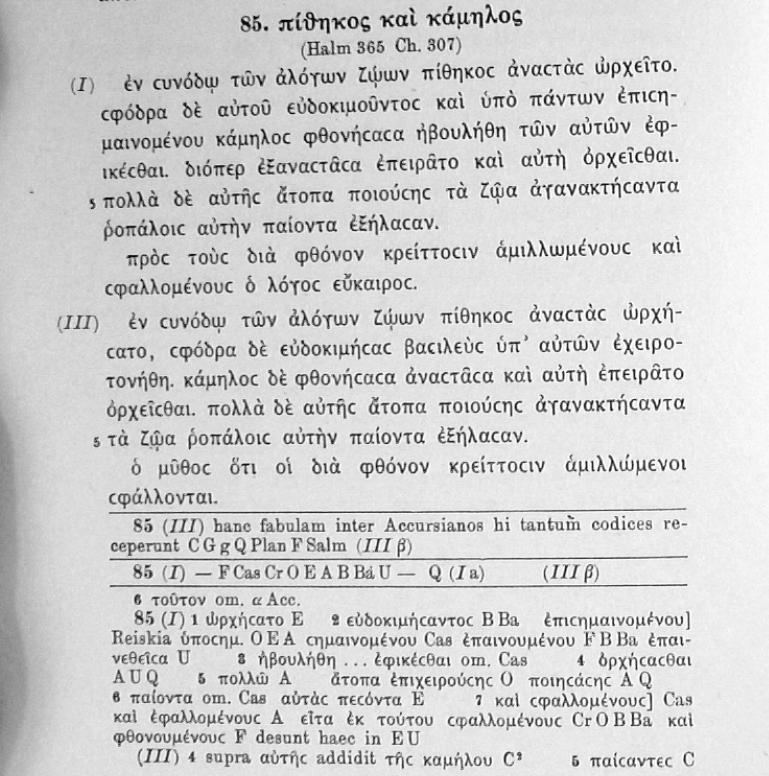
\includegraphics[width=.7\textwidth]{imgs/Edizione-Critica-apparato.png}
    \end{center}

\end{frame}



\begin{frame}
    \frametitle{TEI Modulo 12 - Codifica Edizioni Critiche}
    \framesubtitle{Getting started}
    \addtocounter{nframe}{1}

    
    % * Evidenziazione, page 1
    % Witnesses to a text may include authorial or other manuscripts, printed editions of the work, early translations, or quotations of a work in other texts


    \begin{block}{Edizioni critiche di testi}
        I documenti testimoni di un testo (\textit{tradizione}) possono essere di varia natura:
        \begin{itemize}
            \item manoscritti d'autore
            \item manoscritti copia
            \item edizioni a stampa
            \item traduzioni
            \item citazioni in testimonianze indirette
            \item ...
        \end{itemize}
    \end{block}

\end{frame}

\begin{frame}
    \frametitle{TEI Modulo 12 - Codifica Edizioni Critiche}
    \addtocounter{nframe}{1}
    
    \begin{center}
        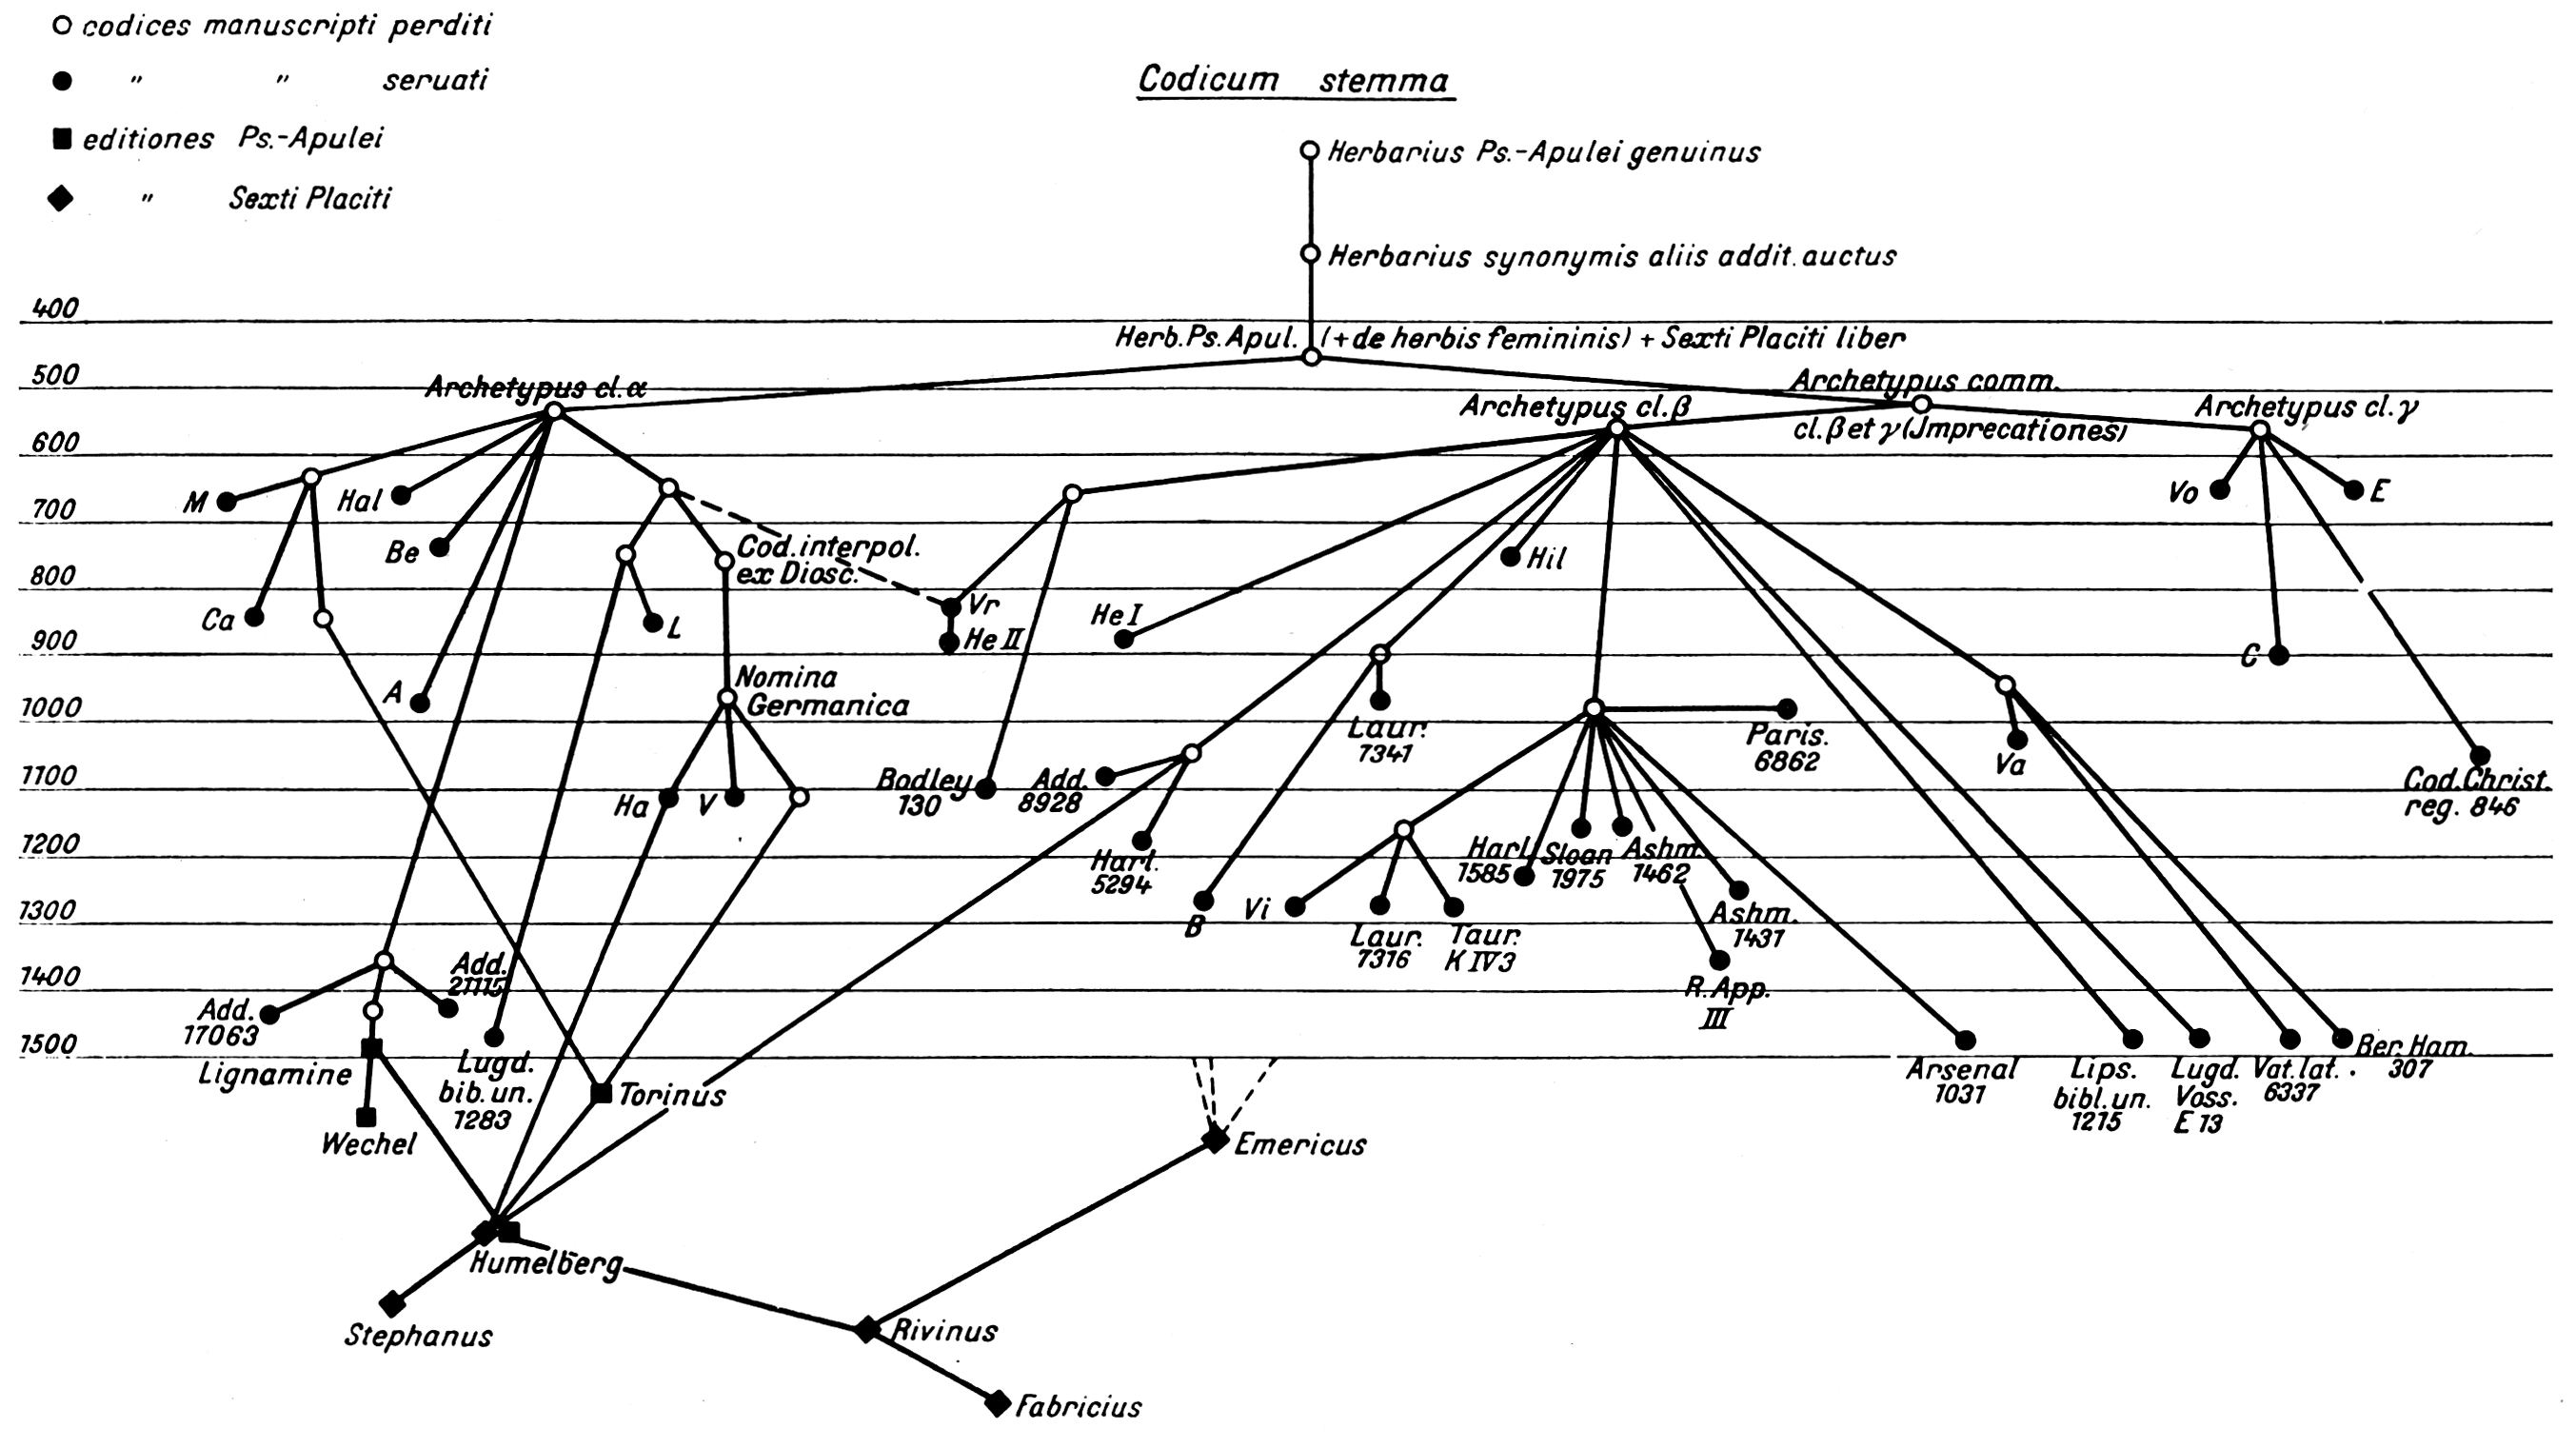
\includegraphics[width=.95\textwidth]{imgs/image.png}
    \end{center}

\end{frame}

\begin{frame}
    \frametitle{TEI Modulo 12 - Codifica Edizioni Critiche}
    \framesubtitle{Getting started}
    \addtocounter{nframe}{1}


    \begin{block}{Cosa rappresenta un apparato critico}
        \begin{itemize}
            \item Rappresentare diverse versioni di uno stesso passo di testo lette da diverse fonti
            \item Accompagnare la scelta dell'editore nel lavoro di ricostruzione del testo
            \item Rappresentare una diramazione del testo nella tradizione e un conseguente ricongiungimento
        \end{itemize}
    \end{block}
       
\end{frame}

\begin{frame}
    \frametitle{TEI Modulo 12 - Codifica Edizioni Critiche}
    \addtocounter{nframe}{1}
    
    \textbf{semplice esempio del grafo delle varianti}

    \begin{center}
        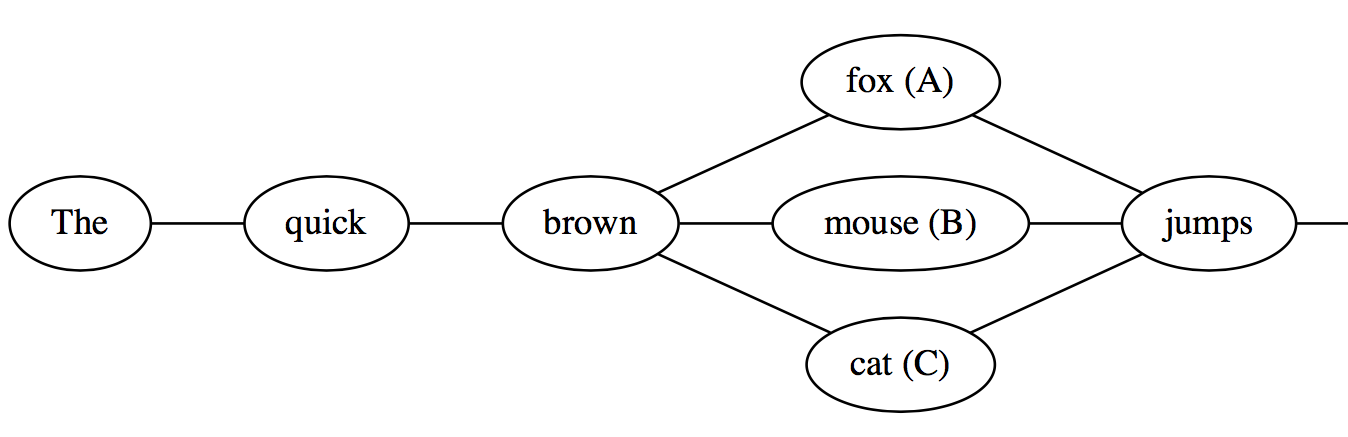
\includegraphics[width=.95\textwidth]{imgs/testo-divergente.png}
    \end{center}

    \textit{image from \url{http://doi.org/10.5281/zenodo.3446155}}

\end{frame}

\begin{frame}
    \frametitle{TEI Modulo 12 - Codifica Edizioni Critiche}
    \framesubtitle{Getting started}
    \addtocounter{nframe}{1}

    % * Evidenziazione, page 1
    % encoding such an apparatus of variants

    % * Evidenziazione, page 1
    % provides extra attributes for some elements of the core tag set when this module is selected
    
    \begin{block}{Obiettivo del modulo 12 (Critical Apparatus)}
        Codificare in forma strutturata l'apparato critico e l'insieme dei testimoni
    \end{block}

    \begin{block}{Modulo 12 delle linee guida TEI}
        Definisce elementi, attributi e prassi per la rappresentazione digitale di edizioni critiche
    \end{block}

\end{frame}

\begin{frame}
    \frametitle{TEI Modulo 12 - Codifica Edizioni Critiche}
    \framesubtitle{Getting started}
    \addtocounter{nframe}{1}

    % * Evidenziazione, page 1
% variant readings

% * Evidenziazione, page 1
% may be recorded in a series of apparatus entries

% * Evidenziazione, page 1
% documentation of the witnesses whose readings are included in the apparatus

    \begin{block}{Modulo 12 delle linee guida TEI}
       Grazie alle specifiche del modulo è possibile registrare la lezione a testo e le lezioni non accolte dei vari testimoni della tradizione
    \end{block}

    \begin{block}{Modulo 12 delle linee guida TEI}
       Documentare i dettagli dei testimoni i quali sono rappresentati con sigle distintive
     \end{block}

\end{frame}

\begin{frame}
    \frametitle{TEI Modulo 12 - Codifica Edizioni Critiche}
    \framesubtitle{Getting started}
    \addtocounter{nframe}{1}


    \begin{block}{Modulo 12 delle linee guida TEI}
        \begin{itemize}
            \item registrare contenuto di testimoni frammentari
            \item registrare le entrate di apparato intercalandole al testo principale (embedded/inline)
            \item registrare le entrate di apparato separate dal testo principale (apparato esterno)
        \end{itemize}
    \end{block}


\end{frame}

\begin{frame}
    \frametitle{TEI Modulo 12 - Codifica Edizioni Critiche}
    \framesubtitle{Apparatus, Readings, Witnesses}
    \addtocounter{nframe}{1}

    % * Evidenziazione, page 1
    % Apparatus

    % * Evidenziazione, page 1
    % Readings

    % * Evidenziazione, page 1
    % Witnesses

    % * Evidenziazione, page 1
    % fundamental markup methods used to encode textual variations

    % * Evidenziazione, page 2
    % the app element for entries in the critical apparatus

    % * Evidenziazione, page 2
    % identifying individual readings

    % * Evidenziazione, page 2
    % ways of grouping readings together

    % * Evidenziazione, page 2
    % identifying which witnesses support a particular reading

    % * Evidenziazione, page 2
    % describing the witnesses included in the apparatus

    % * Evidenziazione, page 2
    % which portions of a text are covered by fragmentary witnesses

    \begin{block}{Elementi fondamentali per la codifica di un testo critico}
        \begin{itemize}
            \item Le singole entrate di apparato sono rappresentate dall'elemento \texttt{<app>}
            \item Le differenti letture sono registrate con l'elemento \texttt{<rdg>}
            \item La lettura accolta a testo è registrata con l'elemento \texttt{<lemma>}
            \item I testimoni sono registrati con l'elemento \texttt{<witness>}
        \end{itemize}
       
    \end{block}


\end{frame}


\begin{frame}
    \frametitle{TEI Modulo 12 - Codifica Edizioni Critiche}
    \framesubtitle{Apparatus, Readings, Witnesses}
    \addtocounter{nframe}{1}

    % * Evidenziazione, page 1
    % Apparatus

    % * Evidenziazione, page 1
    % Readings

    % * Evidenziazione, page 1
    % Witnesses

    % * Evidenziazione, page 1
    % fundamental markup methods used to encode textual variations

    % * Evidenziazione, page 2
    % the app element for entries in the critical apparatus

    % * Evidenziazione, page 2
    % identifying individual readings

    % * Evidenziazione, page 2
    % ways of grouping readings together

    % * Evidenziazione, page 2
    % identifying which witnesses support a particular reading

    % * Evidenziazione, page 2
    % describing the witnesses included in the apparatus

    % * Evidenziazione, page 2
    % which portions of a text are covered by fragmentary witnesses

    \begin{block}{Elementi fondamentali per la codifica di un testo critico}
        \begin{itemize}
            \item Le varianti possono essere raggruppate con l'elemento \texttt{<rgdGrp>}
            \item La tradizione dei testimoni considerati sono raggruppati nell'elemento \texttt{<listWit>}
            \item I testimoni possono essere indicati anche accanto alla variante con l'elemento \texttt{<wit>}
        \end{itemize}
       
    \end{block}

\end{frame}

\begin{frame}
    \frametitle{TEI Modulo 12 - Codifica Edizioni Critiche}
    \framesubtitle{Apparatus, Readings, Witnesses}
    \addtocounter{nframe}{1}

    % * Evidenziazione, page 2
% The app element

% * Evidenziazione, page 2
% The individual apparatus entry is encoded with the app element

% * Evidenziazione, page 2
% a way of marking points where the encoding of a passage in a single source may be carried out in more than one way


% * Evidenziazione, page 2
% Individual textual variations are encoded using the app element

% * Evidenziazione, page 2
% which groups together all the readings constituting the variation

% * Evidenziazione, page 2
% is not a purely mechanical process

% * Evidenziazione, page 2
% Each app element usually comprises one or more readings


    \begin{block}{L'elemento \texttt{<app>}}

        L'elemento distintivo per la codifica delle entrate di apparato nel vocabolario TEI-XML è l'elemento \texttt{app}

    \end{block}
    \begin{block}{L'elemento \texttt{<app>}}

        \begin{itemize}
            \item codificare il contenuto testuale di una fonte in più versioni
            \item codificare variazioni testuali
            \item riunire tutte le lezioni di uno stesso passo testuale
        \end{itemize}

    \end{block}


\end{frame}


\begin{frame}
    \frametitle{TEI Modulo 12 - Codifica Edizioni Critiche}
    \framesubtitle{Apparatus, Readings, Witnesses}
    \addtocounter{nframe}{1}

    % * Evidenziazione, page 2
% several methods may be used for such linkage

    \begin{block}{Metodi per codificare l'apparato critico}
        \begin{itemize}
            \item location-referenced method
            \item double-end-point-attached method
            \item the parallel segmentation method
        \end{itemize}

       
    \end{block}


\end{frame}


\begin{frame}
    \frametitle{TEI Modulo 12 - Codifica Edizioni Critiche}
    \framesubtitle{Apparatus, Readings, Witnesses}
    \addtocounter{nframe}{1}

    % * Evidenziazione, page 2
    % <app> (apparatus entry) contains one entry in a critical apparatus, with an optional lemma and usually one or more readings or notes on the relevant passage.

    % * Evidenziazione, page 2
    % @type

    % * Evidenziazione, page 2
    % classifies the variation contained in this element according to some convenient typology

    % * Evidenziazione, page 2
    % @from

    % * Evidenziazione, page 2
    % identifies the beginning of the lemma in the base text.

    % * Evidenziazione, page 2
    % @to

    % * Evidenziazione, page 2
    % identifies the endpoint of the lemma in the base text.

    % * Evidenziazione, page 2
    % @loc

    % * Evidenziazione, page 2
    % location

    % * Evidenziazione, page 2
    % indicates the location of the variation

    % * Evidenziazione, page 2
    % The attributes @loc, @from, and @to, are used to link the apparatus entry to the base text

    \begin{block}{L'elemento \texttt{<app>}}
        \texttt{<app>} (\textit{apparatus entry}) contains one entry in a critical apparatus, with an optional lemma and usually one or more readings or notes on the relevant passage.
    \end{block}

\end{frame}

\begin{frame}
    \frametitle{TEI Modulo 12 - Codifica Edizioni Critiche}
    \framesubtitle{Apparatus, Readings, Witnesses}
    \addtocounter{nframe}{1}

    % * Evidenziazione, page 2
    % <app> (apparatus entry) contains one entry in a critical apparatus, with an optional lemma and usually one or more readings or notes on the relevant passage.

    % * Evidenziazione, page 2
    % @type

    % * Evidenziazione, page 2
    % classifies the variation contained in this element according to some convenient typology

    % * Evidenziazione, page 2
    % @from

    % * Evidenziazione, page 2
    % identifies the beginning of the lemma in the base text.

    % * Evidenziazione, page 2
    % @to

    % * Evidenziazione, page 2
    % identifies the endpoint of the lemma in the base text.

    % * Evidenziazione, page 2
    % @loc

    % * Evidenziazione, page 2
    % location

    % * Evidenziazione, page 2
    % indicates the location of the variation

    % * Evidenziazione, page 2
    % The attributes @loc, @from, and @to, are used to link the apparatus entry to the base text

    \begin{block}{Attributi significativi dell'elemento \texttt{<app>}}
        \begin{itemize}
            \item \texttt{@type}: \textit{classifies the variation contained in this element according to some convenient typology}
            \item \texttt{@from}: \textit{identifies the beginning of the lemma in the base text.}
            \item \texttt{@to}: \textit{identifies the endpoint of the lemma in the base text}
            \item \texttt{@loc}: \textit{indicates the location of the variation}
        \end{itemize}
    \end{block}

    \textit{Gli attributi @loc, @from, and @to, sono impiegati per collegare l'entrata di apparato al testo principale (esistono vari metodi)}


\end{frame}

\begin{frame}
    \frametitle{TEI Modulo 12 - Codifica Edizioni Critiche}
    \addtocounter{nframe}{1}
    
    % * Evidenziazione, page 2
    % A very simple partial apparatus

    % * Evidenziazione, page 3
    % in practice the apparatus will be somewhat more complex

    \begin{center}
        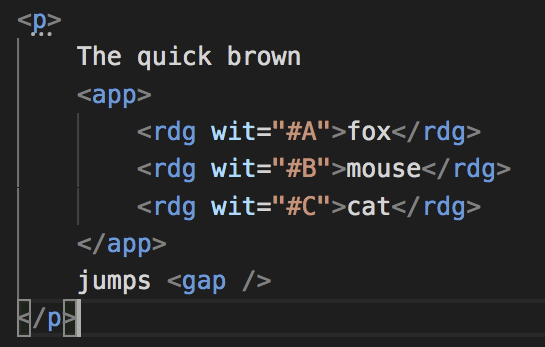
\includegraphics[width=.95\textwidth]{imgs/fox-jumps.png}
    \end{center}

\end{frame}
% * Evidenziazione, page 3
% readings

% * Evidenziazione, page 3
% subvariation

% * Evidenziazione, page 3
% witness information



\begin{frame}
    \frametitle{TEI Modulo 12 - Codifica Edizioni Critiche}
    \framesubtitle{Apparatus, Readings, Witnesses}
    \addtocounter{nframe}{1}

    % * Evidenziazione, page 3
    % Individual readings are the crucial elements in any critical apparatus of variants

    % * Evidenziazione, page 3
    % tag individual readings within an apparatus entry:


    \begin{block}{Registrazione delle diverse lezioni}
        Registrare le singole letture conservate nei singoli testimoni del testo tramandato è l'attività principale per realizzare un apparato delle varianti scientificamente curato 
    \end{block}

    \begin{block}{Registrazione delle diverse lezioni}
        Il vocabolario XML-TEI definisce due elementi per registrare le singole letture 
    \end{block}


\end{frame}


\begin{frame}
    \frametitle{TEI Modulo 12 - Codifica Edizioni Critiche}
    \framesubtitle{Apparatus, Readings, Witnesses}
    \addtocounter{nframe}{1}

% * Evidenziazione, page 3
    % <lem>

    % * Evidenziazione, page 3
    % lemma

    % * Evidenziazione, page 3
    % contains the lemma, or base text, of a textual variation

    % * Evidenziazione, page 3
    % <rdg>

    % * Evidenziazione, page 3
    % reading

    % * Evidenziazione, page 3
    % contains a single reading within a textual variation.

    % * Evidenziazione, page 3
    % the term lemma is used here in the text-critical sense of ‘the reading accepted as that of the original or of the base text’

    \begin{block}{Elementi per la registrazione delle lezioni}
        
        \begin{itemize}
            \item \texttt{<lem>}: \textit{lemma} - contains the lemma, or base text, of a textual variation
            \item \texttt{<rdg>}: \textit{reading} - contains a single reading within a textual variation.
        \end{itemize}

    \end{block}

    \textit{Il termine \textbf{lemma} è inteso nell'accezione di \textbf{lezione accettata dall'editore come lezione a testo, oppure in alternativa come lettura presente nel testo base}}

\end{frame}


\begin{frame}
    \frametitle{TEI Modulo 12 - Codifica Edizioni Critiche}
    \framesubtitle{Apparatus, Readings, Witnesses}
    \addtocounter{nframe}{1}


    % * Evidenziazione, page 3
    % The lem element may also be used to record the base text of the source edition

    % * Evidenziazione, page 3
    % mark the readings of a base witness, to indicate the preference of an editor or encoder for a particular reading, or (e.g. in the case of an external apparatus) to indicate precisely to which portion of the main text the variation applies.

    % * Evidenziazione, page 3
    % may prefer not to use it at all

    \begin{block}{L'elemento \texttt{<lem>}}
        
        \begin{itemize}
            \item Usato per registrare il testo di base riportato nell'edizione di riferimento
            \item Usato per registrare le lezioni del testimone base di collazione
            \item Usato per registrare la lezione accolta a testo dall'editore dell'edizione critica digitale
            \item Usato per per indicare in modo puntuale a quale porzione del testo principale le letture divergenti si riferiscono
            \item Potrebbe non essere utilizzato affatto
        \end{itemize}

    \end{block}

\end{frame}

\begin{frame}
    \frametitle{TEI Modulo 12 - Codifica Edizioni Critiche}
    \addtocounter{nframe}{1}
    

    \begin{center}
        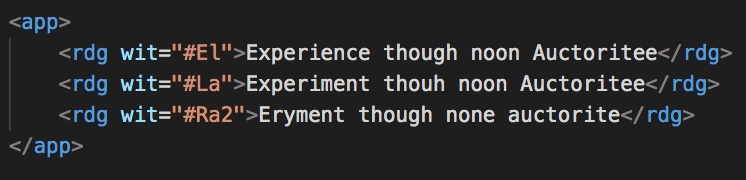
\includegraphics[width=.95\textwidth]{imgs/app-rdg.png}
    \end{center}

\end{frame}


% * Evidenziazione, page 3
% In recording readings within an apparatus entry, the rdg element should always be used; each app usually contains at least one rdg, though it may contain only notes.

% * Evidenziazione, page 3
% How it is used depends in part on the method chosen for linking the apparatus to the text

% * Evidenziazione, page 3
% Readings may be encoded individually, or grouped for perspicuity using the rdgGrp element


\begin{frame}
    \frametitle{TEI Modulo 12 - Codifica Edizioni Critiche}
    \framesubtitle{Apparatus, Readings, Witnesses}
    \addtocounter{nframe}{1}

    \begin{block}{Attributi significativi dell'elemento \texttt{<rdg>} e \texttt{<lem>}}
        \begin{itemize}
            \item \texttt{@wit}: \textit{(witness or witnesses)} - contains a space-delimited list of one or more pointers indicating the witnesses which attest to a given reading
            \item \texttt{@type}: \textit{} - classifies the reading according to some useful typology. Sample values include: 1] \textit{substantive}; 2] \textit{orthographic}
        \end{itemize}
    \end{block}

    \textit{le classi di attributi particolarmente utili sono att.witnessed, att.textCritical, att.global.responsibilit, att.global.source, att.written}

\end{frame}

\begin{frame}
    \frametitle{TEI Modulo 12 - Codifica Edizioni Critiche}
    \framesubtitle{Apparatus, Readings, Witnesses}
    \addtocounter{nframe}{1}

    \begin{block}{Attributi significativi dell'elemento \texttt{<rdg>} e \texttt{<lem>}}
        \begin{itemize}
            \item \texttt{@cause}: \textit{} - classifies the cause for the variant reading, according to any appropriate typology of possible origins. Sample values include: 1] \textit{homeoteleuton}; 2] \textit{homeoarchy}; 3] \textit{paleographicConfusion}; 4] \textit{haplography}; 5] \textit{dittography}; 6] \textit{falseEmendation}
            \item \texttt{@varSeq}: \textit{(variant sequence)} - provides a number indicating the position of this reading in a sequence, when there is reason to presume a sequence to the variants.
        \end{itemize}
    \end{block}

    \textit{le classi di attributi particolarmente utili sono att.witnessed, att.textCritical, att.global.responsibilit, att.global.source, att.written}
    
\end{frame}

\begin{frame}
    \frametitle{TEI Modulo 12 - Codifica Edizioni Critiche}
    \framesubtitle{Apparatus, Readings, Witnesses}
    \addtocounter{nframe}{1}

      
    \begin{block}{Attributi significativi dell'elemento \texttt{<rdg>} e \texttt{lem}}
        \begin{itemize}
            \item \texttt{@hand}: \textit{} - points to a handNote element describing the hand considered responsible for the content of the element concerned
            \item \texttt{@resp}: \textit{(responsible party)} - indicates the agency responsible for the intervention or interpretation, for example an editor or transcriber
            \item \texttt{@source}: \textit{} - specifies the source from which some aspect of this element is drawn
        \end{itemize}
    \end{block}

    \textit{le classi di attributi particolarmente utili sono att.witnessed, att.textCritical, att.global.responsibilit, att.global.source, att.written}

\end{frame}

\begin{frame}
    \frametitle{TEI Modulo 12 - Codifica Edizioni Critiche}
    \framesubtitle{Apparatus, Readings, Witnesses}
    \addtocounter{nframe}{1}

      
    \begin{block}{Attributi significativi dell'elemento \texttt{<rdg>} e \texttt{lem}}
        \begin{itemize}
            \item \texttt{@cert}: \textit{(certainty)} - signifies the degree of certainty associated with the intervention or interpretation
            \item \texttt{@exclude}	\textit{} - points to elements that are in exclusive alternation with the current element.
        \end{itemize}
    \end{block}

    \textit{le classi di attributi particolarmente utili sono att.witnessed, att.textCritical, att.global.responsibilit, att.global.source, att.written}

\end{frame}


\begin{frame}
    \frametitle{TEI Modulo 12 - Codifica Edizioni Critiche}
    \framesubtitle{@hand, @source, @resp, @wit}
    \addtocounter{nframe}{1}

    % * Evidenziazione, page 6
    % Encoders should be aware of the distinct fields of use of the attribute values @wit, @hand, and @source

    % * Evidenziazione, page 6
    % @wit identifies the physical entity in which the reading is found (manuscript, clay tablet, papyrus, printed edition);

    % * Evidenziazione, page 6
    % @hand refers to the agent responsible for inscribing that reading in that physical entity (scribe, author, inscriber, hand 1, hand 2)

    % * Evidenziazione, page 6
    % @source indicates the scholar responsible for asserting the existence of that reading in that physical entity

    \begin{block}{Attributi elementi lezioni}
        \texttt{@wit} identifies the physical entity in which the reading is found (manuscript, clay tablet, papyrus, printed edition)
    \end{block}

    \begin{block}{Attributi elementi lezioni}
        \texttt{@hand} refers to the agent responsible for inscribing that reading in that physical entity (scribe, author, inscriber, hand 1, hand 2) 
    \end{block}


\end{frame}


\begin{frame}
    \frametitle{TEI Modulo 12 - Codifica Edizioni Critiche}
    \framesubtitle{@hand, @source, @resp, @wit}
    \addtocounter{nframe}{1}

    % * Evidenziazione, page 6
    % Encoders should be aware of the distinct fields of use of the attribute values @wit, @hand, and @source

    % * Evidenziazione, page 6
    % @wit identifies the physical entity in which the reading is found (manuscript, clay tablet, papyrus, printed edition);

    % * Evidenziazione, page 6
    % @hand refers to the agent responsible for inscribing that reading in that physical entity (scribe, author, inscriber, hand 1, hand 2)

    % * Evidenziazione, page 6
    % @source indicates the scholar responsible for asserting the existence of that reading in that physical entity

    \begin{block}{Attributi elementi lezioni}
        \texttt{@source} indicates the scholars responsible for asserting the existence of that reading in that physical entity
    \end{block}

    \begin{block}{Attributi elementi lezioni}
         \texttt{@resp} indicates the scholars responsible for supplying the intellectual content of the reading reported in the transcription
    \end{block}

\end{frame}

%%%% ESEMPI IMMAGINI %%%%
%%                     %%

\begin{frame}
    \frametitle{TEI Modulo 12 - Codifica Edizioni Critiche}
    \addtocounter{nframe}{1}
        
    \begin{center}
        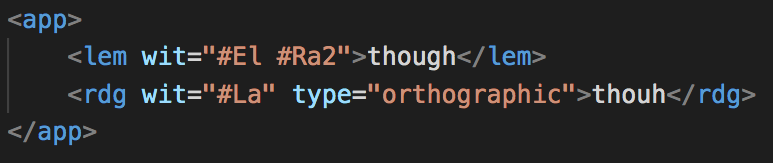
\includegraphics[width=.95\textwidth]{imgs/1-rdg-type.png}
    \end{center}

\end{frame}

\begin{frame}
    \frametitle{TEI Modulo 12 - Codifica Edizioni Critiche}
    \addtocounter{nframe}{1}
        
    \begin{center}
        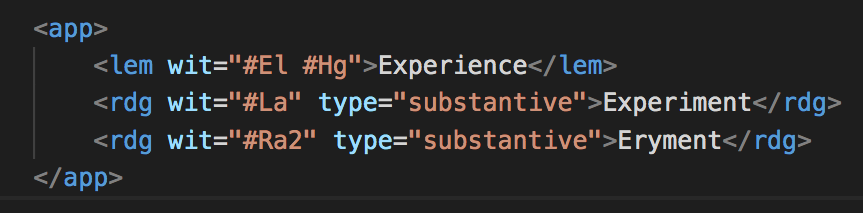
\includegraphics[width=.95\textwidth]{imgs/2-lem-rdg.png}
    \end{center}

\end{frame}

\begin{frame}
    \frametitle{TEI Modulo 12 - Codifica Edizioni Critiche}
    \addtocounter{nframe}{1}
        
    \begin{center}
        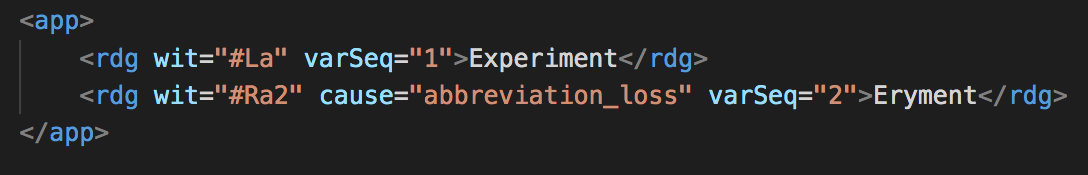
\includegraphics[width=.95\textwidth]{imgs/3-app-cause-varSeq.png}
    \end{center}

\end{frame}

\begin{frame}
    \frametitle{TEI Modulo 12 - Codifica Edizioni Critiche}
    \addtocounter{nframe}{1}
        
    \begin{center}
        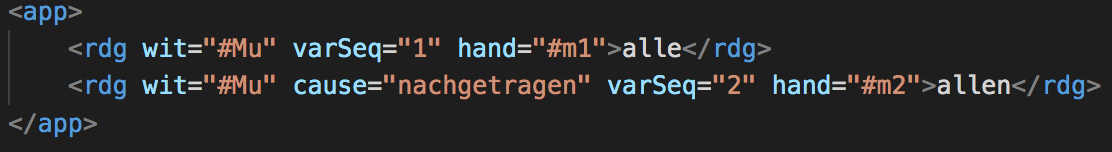
\includegraphics[width=.95\textwidth]{imgs/4-nachgetragen-aggiunta.png}
    \end{center}

\end{frame}

\begin{frame}
    \frametitle{TEI Modulo 12 - Codifica Edizioni Critiche}
    \addtocounter{nframe}{1}
        
    \begin{center}
        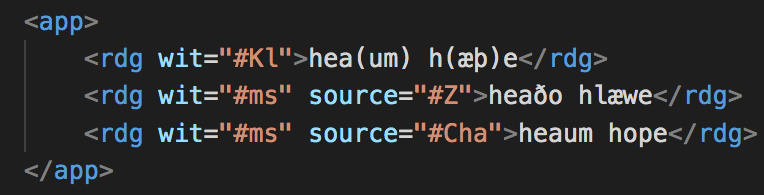
\includegraphics[width=.95\textwidth]{imgs/5-rdg-source.png}
    \end{center}

\end{frame}

% * Evidenziazione, page 6
% Where there is a greater weight of editorial discussion and interpretation

% * Evidenziazione, page 6
% this information can be attached to the apparatus in a note.

% * Evidenziazione, page 6
% The note element may also be used to record the specific wording of notes in the apparatus of the source edition

% * Evidenziazione, page 6
% <note source="#Kl">

% * Evidenziazione, page 6
% Notes providing details of the reading of one particular witness should be encoded using the specialized witDetail element



% * Evidenziazione, page 6
% the categories may blur: a scholar may produce an edition introducing readings for which he or she is responsible; that edition may itself become a witness in a later critical apparatus.





\begin{frame}
    \frametitle{TEI Modulo 12 - Codifica Edizioni Critiche}
    \framesubtitle{raggruppamento di lezioni e subvariation}
    \addtocounter{nframe}{1}

    % * Evidenziazione, page 6
% Subvariation

% * Evidenziazione, page 6
% The rdgGrp element may be used to group readings

% * Evidenziazione, page 6
% they have identical values on one or more attributes, or because they are seen as forming a self-contained variant sequence, or for some other reason

    \begin{block}{raggruppare diverse lezioni}
        E' possibile raggruppare diverse lezioni con l'elemento \texttt{<rdgGrp>}
    \end{block}

    \begin{itemize}
        \item se più lezioni hanno identici valori per uno o più attributi
        \item se più lezioni sono in relazione d'ordine tra lavoro
        \item se più lezioni hanno un qualche tipo di relazione
    \end{itemize}

\end{frame}


\begin{frame}
    \frametitle{TEI Modulo 12 - Codifica Edizioni Critiche}
    \framesubtitle{raggruppamento di lezioni e subvariation}
    \addtocounter{nframe}{1}

    % * Evidenziazione, page 7
    % <rdgGrp>

    % * Evidenziazione, page 7
    % reading group

    % * Evidenziazione, page 7
    % groups two or more readings perceived to have a genetic relationship or other affinity

    % * Evidenziazione, page 7
    % The rdgGrp element is a member of class att.textCritical and therefore can carry the @wit, @type, @cause, @varSeq, @hand, and @resp attributes described in the preceding section.

   

    \begin{block}{raggruppare diverse lezioni}
        \texttt{<rdgGrp>} \textit{(reading group)} - within a textual variation, groups two or more readings perceived to have a genetic relationship or other affinity.
    \end{block}

    \begin{center}
       L'elemento \texttt{rdgGrp} può essere caratterizzato dagli stessi attributi dell'elemento \texttt{lem} e dell'elemento \texttt{rdg} \textit{@wit, @type, @cause, @varSeq, @hand, @source, @resp, @exclude}
    \end{center}

\end{frame}


\begin{frame}
    \frametitle{TEI Modulo 12 - Codifica Edizioni Critiche}
    \framesubtitle{raggruppamento di lezioni e subvariation}
    \addtocounter{nframe}{1}

    % * Evidenziazione, page 7
    % When values for any of these attributes are given on a rdgGrp element, the values given are inherited by the rdg or lem elements nested within the reading group
   

    \begin{block}{raggruppare diverse lezioni}
        I valori degli attributi se associati all'elemento \texttt{rdgGrp} vengono ereditati dagli elementi annidati nel gruppo \texttt{rdg} e \texttt{lem}.
    \end{block}


\end{frame}

 

\begin{frame}
    \frametitle{TEI Modulo 12 - Codifica Edizioni Critiche}
    \framesubtitle{raggruppamento di lezioni e subvariation}
    \addtocounter{nframe}{1}
    
    % * Evidenziazione, page 7
    % To indicate that both Hg and La vary only orthographically from the lemma, one might tag both readings <rdg type='orthographic'>

    % * Evidenziazione, page 7
    % This fact can be expressed more perspicuously, however, by grouping their readings into a rdgGrp

    % * Evidenziazione, page 7
    % <app> <lem wit="#El #Ra2">though</lem> <rdgGrp type="orthographic"> <rdg wit="#La">thogh</rdg> <rdg wit="#Hg">thouh</rdg> </rdgGrp> </app>

    \begin{center}
        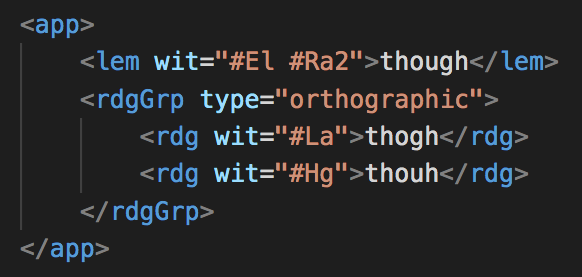
\includegraphics[width=.95\textwidth]{imgs/rdgGrp.png}
    \end{center}


\end{frame}



\begin{frame}
    \frametitle{TEI Modulo 12 - Codifica Edizioni Critiche}
    \framesubtitle{raggruppamento di lezioni e subvariation}
    \addtocounter{nframe}{1}

   % * Evidenziazione, page 7
    % Similarly, rdgGrp may be used to organize the substantive variants of an apparatus entry.

    % * Evidenziazione, page 7
    % Editors may need to indicate that each of a group of witnesses may be taken as all supporting a particular reading

    % * Evidenziazione, page 7
    % manuscripts display many different spellings of these words

    % * Evidenziazione, page 7
    % all these variant spellings and that these variant spellings actually support only the three regularized spelling forms

    % * Evidenziazione, page 7
    % One may term these variant spellings as ‘subvariants’ of the regularized spelling forms.

    % * Evidenziazione, page 7
    % This subvariation can be expressed within an app element by gathering the readings into three groups according to the normalized form of their reading.

    % * Evidenziazione, page 7
    % All the readings within each group may be accounted subvariants of the main reading for the group

    % * Evidenziazione, page 7
    % tagging it as a lem element or as <rdg type='groupBase'>


    \begin{block}{raggruppare diverse lezioni}
        \begin{itemize}
            \item \texttt{rgdGrp} può essere utilizzato per raggruppare varianti sostanziali e sottovarianti formali
            \item indicare diverse varianti formali che supportano la stessa variante sostanziale
            \item codificare ciascuna variante sostanziale con l'elemento \texttt{lem} e le varianti formali con l'elemento \texttt{rdg}, tutto all'interno di un elemento \texttt{rdgGrp}
        \end{itemize}
    \end{block}

\end{frame}


\begin{frame}
    \frametitle{TEI Modulo 12 - Codifica Edizioni Critiche}
    \framesubtitle{raggruppamento di lezioni e subvariation}
    \addtocounter{nframe}{1}
    
    % * Evidenziazione, page 7
    % In this example, the different subvariants on Experience, Experiment, and Eriment are held within three rdgGrp elements nested within the enclosing app element:



    % * Evidenziazione, page 8
    % From this, one may deduce that the regularized reading Experience is supported by all three manuscripts El Hg Ha4, although the spelling differs in Ha4, and that the regularized reading Eriment is supported by Ra2, even though the form differs in that manuscript.

    % * Evidenziazione, page 8
    % Thus, Ha4 here supports the reading Experience found in El and Hg, even though it is spelt slightly differently in Ha4.

    % * Evidenziazione, page 8
    % Reading groups may nest recursively, so that variants can be classified to any desired depth.
    

    \begin{center}
        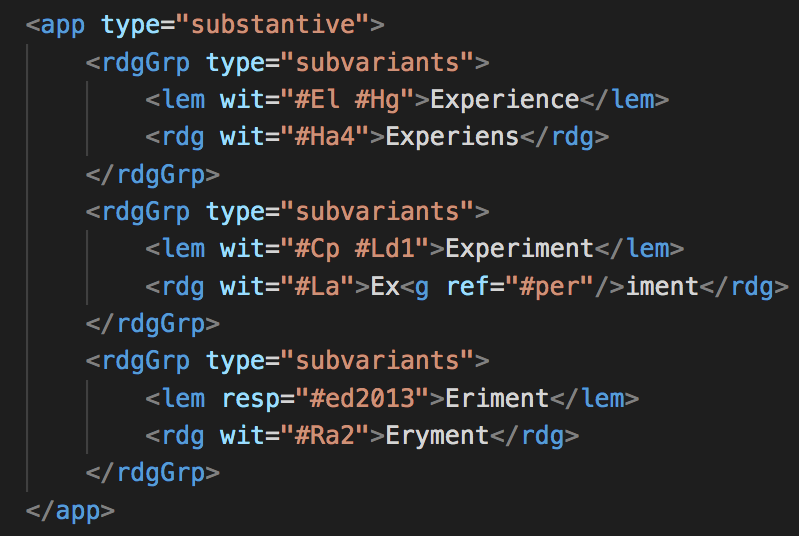
\includegraphics[width=.95\textwidth]{imgs/variant-subvariant.png}
    \end{center}


\end{frame}



\begin{frame}
    \frametitle{TEI Modulo 12 - Codifica Edizioni Critiche}
    \framesubtitle{raggruppamento di lezioni e subvariation}
    \addtocounter{nframe}{1}

  
    % * Evidenziazione, page 8
    % Because apparatus entries may also nest, the app element might also be used to group readings in the same way.

    \begin{block}{raggruppare diverse lezioni}
       Le entrate di apparato, definite con l'elemento \texttt{<app>}  possono essere annidate l'una nell'altra.
    \end{block}
    \begin{block}{raggruppare diverse lezioni}
        Anche l'elemento \texttt{<app>} può essere usato per raggruppare diverse letture seguendo qualche tipo di classificazione.
     \end{block}


\end{frame}



\begin{frame}
    \frametitle{TEI Modulo 12 - Codifica Edizioni Critiche}
    \framesubtitle{raggruppamento di lezioni e subvariation}
    \addtocounter{nframe}{1}
    
    % * Evidenziazione, page 8
    % this variation has three normalized readings, and that the first of these is supported by manuscripts El, Hg, and Ha4; the second by Cp, Ld1, and La; and the third by Ra2

    \begin{center}
        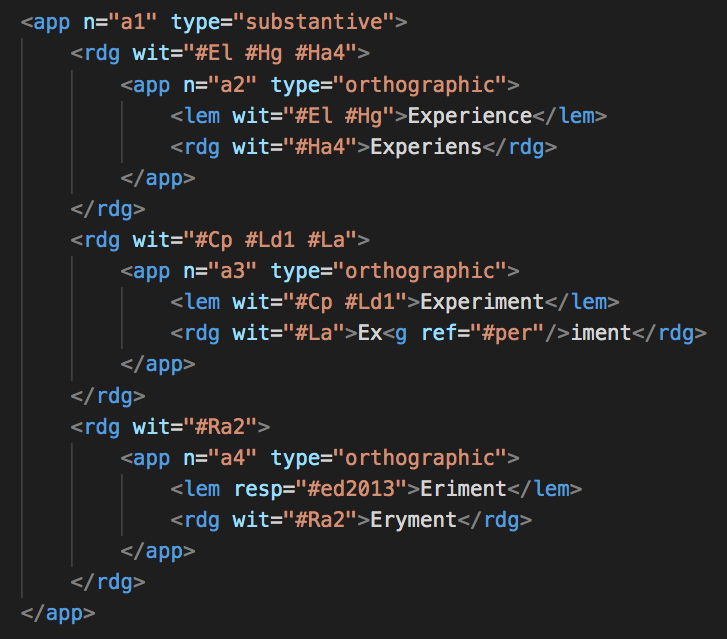
\includegraphics[width=.80\textwidth]{imgs/nest-app.png}
    \end{center}


\end{frame}

\begin{frame}
    \frametitle{TEI Modulo 12 - Codifica Edizioni Critiche}
    \framesubtitle{raggruppamento di lezioni e subvariation}
    \addtocounter{nframe}{1}
    
    % * Evidenziazione, page 8
    % Reading groups may also be used to bring together variants which form an apparent developmental sequence

    \begin{center}
        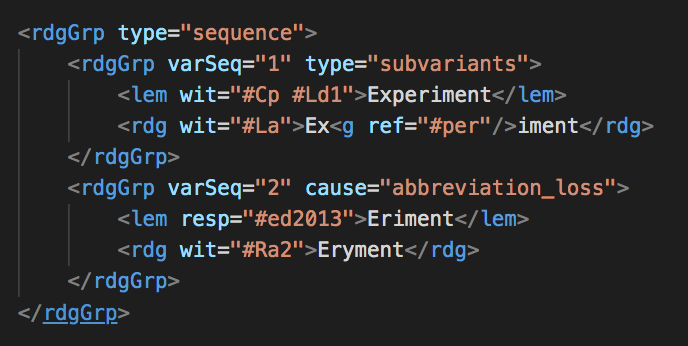
\includegraphics[width=.95\textwidth]{imgs/rdgGrp-seq.png}
    \end{center}


\end{frame}



\begin{frame}
    \frametitle{TEI Modulo 12 - Codifica Edizioni Critiche}
    \framesubtitle{descrizione dei testimoni}
    \addtocounter{nframe}{1}

    \begin{block}{informazioni su singoli testimoni}
      \begin{itemize}
          \item Associare specifiche informazioni relative ad un testimone tra quelli che concordano sulla stessa lezione
          \item Trascrivere letteralmente le informazioni presenti su un testimone da un edizione di riferimento
          \item Definire l'insieme (più o meno strutturato) dei testimoni recensiti
      \end{itemize}
    \end{block}

\end{frame}



\begin{frame}
    \frametitle{TEI Modulo 12 - Codifica Edizioni Critiche}
    \framesubtitle{descrizione dei testimoni}
    \addtocounter{nframe}{1}

    % * Evidenziazione, page 9
    % A given reading is associated with the set of witnesses attesting it by listing the witnesses in the @wit attribute on the rdg or lem element

    % * Evidenziazione, page 9
    % associate annotation on a reading with one specific witness among several

    % * Evidenziazione, page 9
    % can be linked to both a reading and to one or more of the witnesses for that reading


    \begin{block}{elemento \texttt{<witDetail>}}
     \texttt{<witDetail>} \textit{(witness detail)} - gives further information about a particular witness, or witnesses, to a particular reading
    \end{block}

    \begin{block}{attributi dell'elemento \texttt{<witDetail>}}
        \begin{itemize}
            \item \texttt{@target} \textit{} - specifies the destination of the reference by supplying one or more URI References
            \item \texttt{@wit} \textit{(witnesses)} - indicates the sigil or sigla identifying the witness or witnesses to which the detail refers
        \end{itemize}

    \end{block}

\end{frame}




\begin{frame}
    \frametitle{TEI Modulo 12 - Codifica Edizioni Critiche}
    \framesubtitle{Informazioni sui testimoni}
    \addtocounter{nframe}{1}
    
    % * Evidenziazione, page 8
    % Reading groups may also be used to bring together variants which form an apparent developmental sequence
    % * Evidenziazione, page 9


    % * Evidenziazione, page 9
    % made explicit by the @target attribute

    % * Evidenziazione, page 9
    % the link to the witness, by the @wit attribute

    % * Evidenziazione, page 9
    % @target specifies the destination of the reference

    % * Evidenziazione, page 9
    % @wit (witnesses) indicates the sigil or sigla identifying the witness or witnesses to which the detail refers

    % * Evidenziazione, page 9
    % he witDetail refers to multiple readings, @target must be used to point to the reading(s) being annotated
    
    \begin{center}
        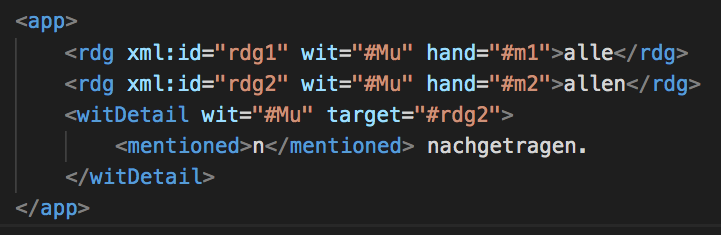
\includegraphics[width=.95\textwidth]{imgs/witDetails.png}
    \end{center}

    % * Evidenziazione, page 10
    % may be used to record the specific wording of information in the source text

    % * Evidenziazione, page 10
    % to record the wording of the note explaining that the variant reading adds n to the original in a second hand

\end{frame}





\begin{frame}
    \frametitle{TEI Modulo 12 - Codifica Edizioni Critiche}
    \framesubtitle{descrizione dei testimoni}
    \addtocounter{nframe}{1}


    \begin{block}{Registrale informazioni sui testimoni}
        \texttt{<wit>} \textit{} - contains a list of one or more sigla of witnesses attesting a given reading, in a textual variation.
    \end{block}

    \begin{center}
        \textit{Usare l'attributo \texttt{@wit} (assieme all'elemento \texttt{<witDetail>} quando necessario) è quasi sempre la scelta più conveniente}
    \end{center}
    
    % * Evidenziazione, page 11
    % @wit is more succinct,

    % * Evidenziazione, page 11
    % using @wit (with witDetail when needed) is almost always to be preferred
\end{frame}

\begin{frame}
    \frametitle{TEI Modulo 12 - Codifica Edizioni Critiche}
    \framesubtitle{Informazioni sui testimoni}
    \addtocounter{nframe}{1}
    
    % * Nota ancorata, page 10
    % nota sigla 

    %The Latin word siglum (sign), pl. sigla denotes the abbreviation used in a critical apparatus to indicate a particular witness

    % * Evidenziazione, page 10
    % lists of sigla

    % * Evidenziazione, page 10
    % may be complex enough

    % * Evidenziazione, page 10
    % in the transcription of printed critical editions, it may be desirable to retain for future reference the exact form in which the source edition records the witnesses to a particular reading;

    % * Evidenziazione, page 10
    % The wit element may be used to transcribe such lists of witnesses to a particular reading.

    % * Evidenziazione, page 10
    % <wit> contains a list of one or more sigla of witnesses attesting a given reading, in a textual variation.

    % * Evidenziazione, page 10
    % The wit list may appear following a rdg, rdgGrp, or lem element in any apparatus entry

    % * Evidenziazione, page 10
    % wit may be used in a way functionally equivalent to @wit if the sigla therein are wrapped in refs with @target attributes pointing to a predefined witness

    
    \begin{center}
        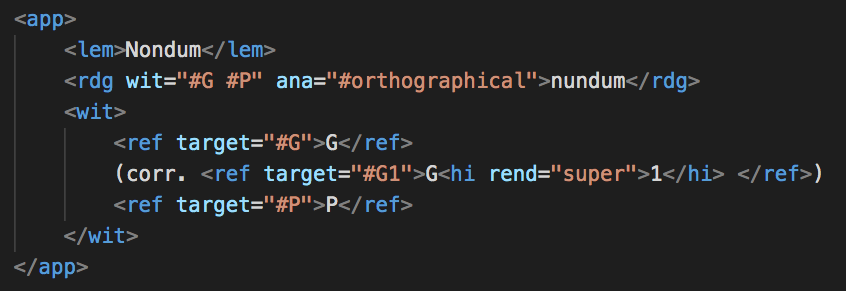
\includegraphics[width=.95\textwidth]{imgs/app-wit.png}
    \end{center}

\end{frame}



\begin{frame}
    \frametitle{TEI Modulo 12 - Codifica Edizioni Critiche}
    \framesubtitle{descrizione dei testimoni}
    \addtocounter{nframe}{1}

    % * Evidenziazione, page 11
    % A list of all identified witnesses should normally be supplied in the front matter of the edition, or in the sourceDesc element of its header

    % * Evidenziazione, page 11
    % may be given either as a simple bibliographic list

    % * Evidenziazione, page 11
    % or as a listWit element,

    % * Evidenziazione, page 11
    % which contains a series of witness elements

    % * Evidenziazione, page 11
    % Each witness element may contain a brief characterization of the witness, given as one or more prose paragraphs
    
    \begin{block}{Insieme dei testimoni recensiti}
        La lista dei testimoni recensita può essere registrata con l'elemento \texttt{<listWit>}
    \end{block}

    \begin{center}{...}
        l'elemento \texttt{<listWit>} contiene a sua volta elementi \texttt{<witness>}. Ciascun elemento \texttt{witness} contiene una breve descrizione del testimone in una forma semi-strutturata. 
    \end{center}
    
   
\end{frame}


\begin{frame}
    \frametitle{TEI Modulo 12 - Codifica Edizioni Critiche}
    \framesubtitle{descrizione dei testimoni}
    \addtocounter{nframe}{1}

    
    \begin{block}{elemento \texttt{<listWit>}}
        \texttt{<listWit>} \textit{(witness list)} - lists definitions for all the witnesses referred to by a critical apparatus, optionally grouped hierarchically.
    \end{block}

    \begin{center}{elemento \texttt{<witness>}}
        \texttt{<witness>} contains either a description of a single witness referred to within the critical apparatus, or a list of witnesses which is to be referred to by a single sigil.
    \end{center}
    
    \textit{La lista dei testimoni è quindi l'insieme delle sigle di tutti i testimoni recensiti e riferiti in apparato}
   
\end{frame}


\begin{frame}
    \frametitle{TEI Modulo 12 - Codifica Edizioni Critiche}
    \framesubtitle{Informazioni sui testimoni}
    \addtocounter{nframe}{1}
    
    
    \begin{center}
        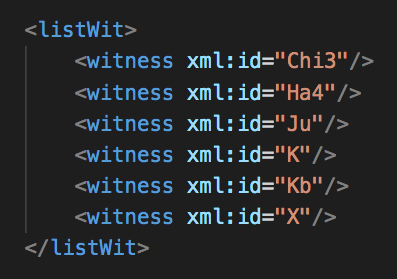
\includegraphics[width=.95\textwidth]{imgs/listWit-base.png}
    \end{center}

\end{frame}


\begin{frame}
    \frametitle{TEI Modulo 12 - Codifica Edizioni Critiche}
    \framesubtitle{Informazioni sui testimoni}
    \addtocounter{nframe}{1}
    
    % * Evidenziazione, page 12
    % each witness element should contain at least a brief prose description of the witness

    % * Evidenziazione, page 12
    % including a bibliographic citation


    % * Evidenziazione, page 12
    % the witness description here may be complemented by a reference to a full description of the manuscript supplied elsewhere, typically as the content of a msDesc or bibl element

    \begin{center}
        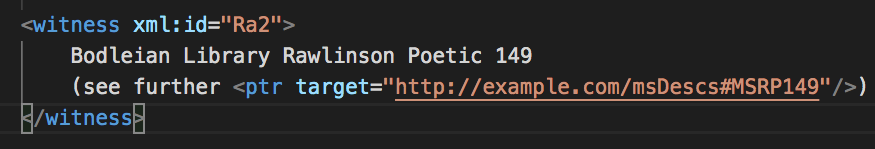
\includegraphics[width=.95\textwidth]{imgs/witness-ref.png}
    \end{center}

    \begin{center}
        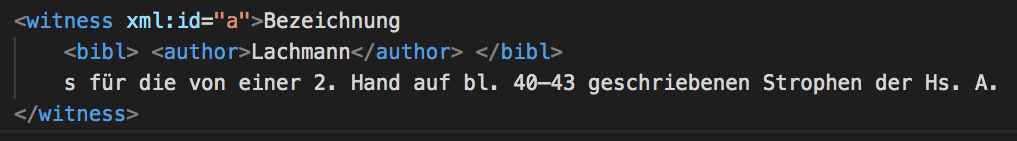
\includegraphics[width=.95\textwidth]{imgs/witness-bibl.png}
    \end{center}

    % * Evidenziazione, page 12
    % a whole paragraph of commentary for each witnes

    % * Evidenziazione, page 13
    % It would however generally be preferable to represent such detailed information using an appropriately structured msDesc element

    % * Evidenziazione, page 13
    % if the witnesses being recorded are not manuscripts but printed works, it may be preferable to document them using the standard bibl or biblStruct elements

\end{frame}




\begin{frame}
    \frametitle{TEI Modulo 12 - Codifica Edizioni Critiche}
    \framesubtitle{descrizione dei testimoni}
    \addtocounter{nframe}{1}

    % * Evidenziazione, page 13
    % In text-critical work it is customary to refer to frequently occurring groups of witnesses by means of a single common siglum

    % * Evidenziazione, page 13
    % including a nested witness list within the witness list

    % * Evidenziazione, page 13
    % uses the siglum for the group as its identifier

    % * Evidenziazione, page 13
    % supplies a fuller name for the group in its optional child head element
    
    \begin{block}{famiglie di testimoni}
        Spesso è utile raggruppare i testimoni in famiglie o in altri tipi di gruppi che riuniscano testimoni con attributi comuni.
    \end{block}
    \begin{block}{famiglie di testimoni}
        Ciò è possibile realizzarlo annidando elementi \texttt{listWit} in altri elementi \texttt{listWit}
    \end{block}
   
\end{frame}


\begin{frame}
    \frametitle{TEI Modulo 12 - Codifica Edizioni Critiche}
    \framesubtitle{Informazioni sui testimoni}
    \addtocounter{nframe}{1}
    
    \begin{center}
        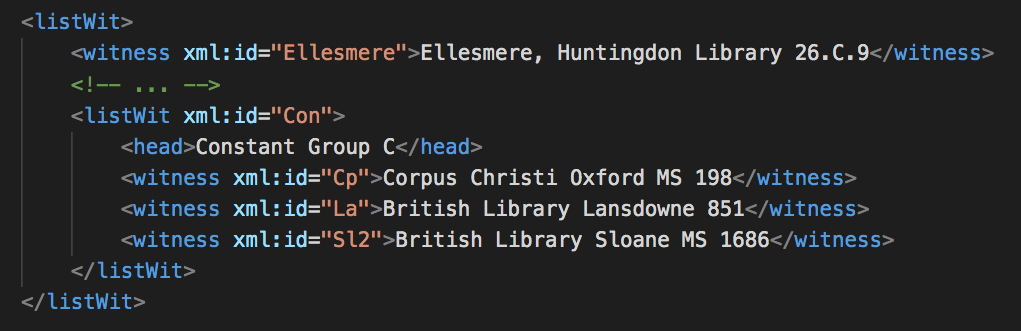
\includegraphics[width=.95\textwidth]{imgs/listWit-nest.png}
    \end{center}


\end{frame}

% * Evidenziazione, page 13
% The more elaborate example below shows both multiple levels of nesting and a strategy for mapping the the @xml:id of the witness to the siglum which will be displayed to the reader of a derived visualisation

% * Evidenziazione, page 13
% <witness xml:id="Σ">Servius (<abbr type="siglum">Σ</abbr>) = ΔΓ

% * Evidenziazione, page 13
% <witness xml:id="Δ">

% * Evidenziazione, page 14
% <abbr type="siglum">Δ</abbr>

% * Evidenziazione, page 14
% <witness xml:id="Γ">

% * Evidenziazione, page 14
% <abbr type="siglum">Γ</abbr>

% * Evidenziazione, page 15
% Here we have a summary of the witnesses, with their sigla, used in an edition, as is generally found in the conspectus siglorum in the front matter of a critical edition.

% * Evidenziazione, page 15
% Families are indicated with Greek letters and manuscript witnesses with Latin letters

% * Evidenziazione, page 15
% The siglum for display is always contained in the abbr with @type ‘siglum’



% * Evidenziazione, page 15
% Situations commonly arise where there are many more or less fragmentary witnesses

% * Evidenziazione, page 15
% there may be quite distinct groups of witnesses for different parts of a text or collection of texts

% * Evidenziazione, page 15
% If a witness list is provided, it may be unnecessary to give, in each apparatus entry, an exhaustive list of the witnesses which agree with the base text

% * Evidenziazione, page 15
% hence calculate all the manuscripts agreeing with the base text

% * Evidenziazione, page 15
% encoders may find it less error-prone to list all witnesses explicitly in each apparatus entry



\begin{frame}
    \frametitle{TEI Modulo 12 - Codifica Edizioni Critiche}
    \framesubtitle{Informazioni sui testimoni}
    \addtocounter{nframe}{1}
    
    \begin{block}{Testimoni frammentari}
       % 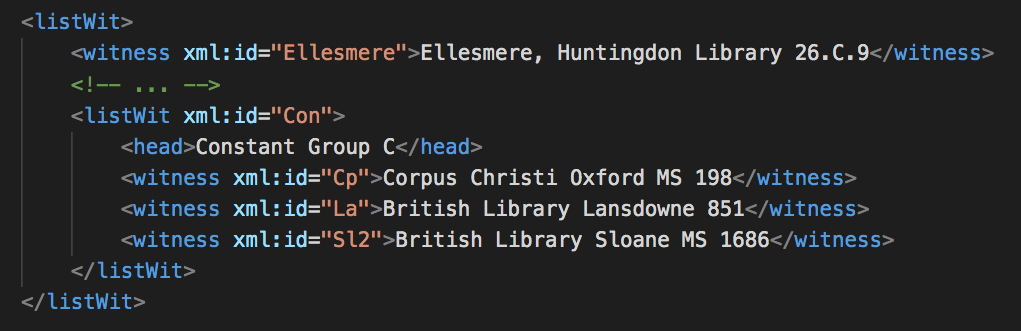
\includegraphics[width=.95\textwidth]{imgs/listWit-nest.png}
       Le linee guida della TEI definiscono alcuni elementi per registrare in apparato testimoni frammentari
    \end{block}

    \begin{block}{Testimoni frammentari}
        all'interno di elementi \texttt{lem} oppure elementi \texttt{rdg} si può registrare l'inizio o la fine di un testimone frammentario ovvero l'inizio o la fine di una lacuna
     \end{block}


\end{frame}

\begin{frame}
    \frametitle{TEI Modulo 12 - Codifica Edizioni Critiche}
    \framesubtitle{Informazioni sui testimoni}
    \addtocounter{nframe}{1}

    
    \begin{block}{Testimoni frammentari}
       % 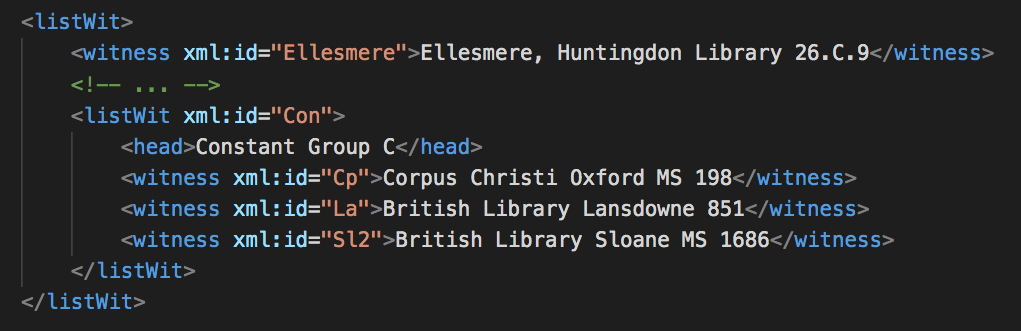
\includegraphics[width=.95\textwidth]{imgs/listWit-nest.png}

       \begin{itemize}
           \item \texttt{<witStart>} \textit{(fragmented witness start)} - indicates the beginning, or resumption, of the text of a fragmentary witness.
           \item \texttt{<witEnd>} \textit{(fragmented witness end)} -  indicates the end, or suspension, of the text of a fragmentary witness.
           \item \texttt{<lacunaStart>} indicates the beginning of a lacuna in the text of a mostly complete textual witness.
           \item \texttt{<lacunaEnd>} indicates the end of a lacuna in a mostly complete textual witness.
       \end{itemize}
      
    \end{block}


\end{frame}



\begin{frame}
    \frametitle{TEI Modulo 12 - Codifica Edizioni Critiche}
    \framesubtitle{Informazioni sui testimoni}
    \addtocounter{nframe}{1}
    
    % * Evidenziazione, page 16
    % In an apparatus this might appear thus, distinguished from the reading of other manuscripts by the presence of the lacunaEnd element:

    % * Evidenziazione, page 16
    % <app> <lem wit="#El #Hg">Auctoritee</lem> <rdg wit="#La #Ra2">auctorite</rdg> <rdg wit="#X"> <lacunaEnd/>auctorite</rdg> </app>

    % * Evidenziazione, page 16
    % <app> <lem wit="#El #Hg">Auctoritee</lem> <rdg wit="#La #Ra2 #X"> <lacunaEnd wit="#X"/>auctorite</rdg> </app>

    % * Evidenziazione, page 16
    % In some cases, the apparatus in the source may commence recording the readings for a particular witness without its being clear whether the previous absence of readings for this witness is due to a lacuna

    % * Evidenziazione, page 16
    % The witStart element may be used in this circumstance:

    % * Evidenziazione, page 16
    % <app> <lem wit="#El #Hg">Auctoritee</lem> <rdg wit="#La #Ra2">auctorite</rdg> <rdg wit="#X"> <witStart/>auctorite</rdg> </app>

    \begin{block}{Testimoni frammentari}
       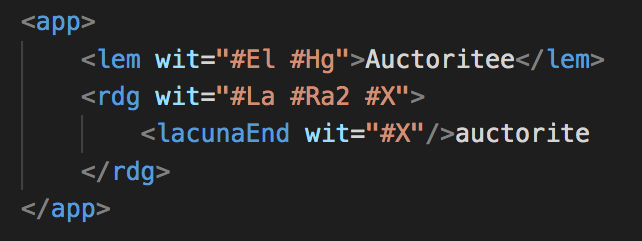
\includegraphics[width=.95\textwidth]{imgs/rdg-lacunaEnd.png}
    \end{block}



\end{frame}

\begin{frame}
    \frametitle{TEI Modulo 12 - Codifica Edizioni Critiche}
    \framesubtitle{Informazioni sui testimoni}
    \addtocounter{nframe}{1}
    
    % * Evidenziazione, page 16
    % In an apparatus this might appear thus, distinguished from the reading of other manuscripts by the presence of the lacunaEnd element:

    % * Evidenziazione, page 16
    % <app> <lem wit="#El #Hg">Auctoritee</lem> <rdg wit="#La #Ra2">auctorite</rdg> <rdg wit="#X"> <lacunaEnd/>auctorite</rdg> </app>

    % * Evidenziazione, page 16
    % <app> <lem wit="#El #Hg">Auctoritee</lem> <rdg wit="#La #Ra2 #X"> <lacunaEnd wit="#X"/>auctorite</rdg> </app>

    % * Evidenziazione, page 16
    % In some cases, the apparatus in the source may commence recording the readings for a particular witness without its being clear whether the previous absence of readings for this witness is due to a lacuna

    % * Evidenziazione, page 16
    % The witStart element may be used in this circumstance:

    % * Evidenziazione, page 16
    % <app> <lem wit="#El #Hg">Auctoritee</lem> <rdg wit="#La #Ra2">auctorite</rdg> <rdg wit="#X"> <witStart/>auctorite</rdg> </app>


    \begin{block}{Testimoni frammentari}
        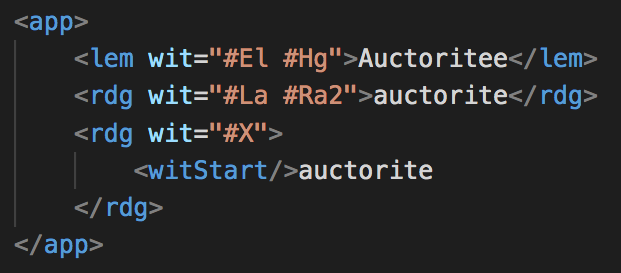
\includegraphics[width=.95\textwidth]{imgs/rdg-witStart.png}
     \end{block}


\end{frame}


\begin{frame}
    \frametitle{TEI Modulo 12 - Codifica Edizioni Critiche}
    \framesubtitle{Collegare l'apparato critico al testo}
    \addtocounter{nframe}{1}
    
    % * Evidenziazione, page 16
    % the location-referenced method,

    % * Evidenziazione, page 16
    % the double-end-point-attached method

    % * Evidenziazione, page 16
    % the parallel segmentation method

    
    \begin{block}{Three diversi metodi per codificare un apparato critico}
       \begin{itemize}
           \item the location-referenced method
           \item the double-end-point-attached method
           \item the parallel segmentation method
       \end{itemize}
     \end{block}


\end{frame}


\begin{frame}
    \frametitle{TEI Modulo 12 - Codifica Edizioni Critiche}
    \framesubtitle{link a critical apparatus to the text}
    \addtocounter{nframe}{1}
    
    \begin{block}{Tre metodi per codificare l'apparato critico}
       \begin{itemize}
           \item \textit{in-line or external apparatus}
           \begin{itemize}
             \item All'interno oppure esternamente al documento che registra il testo di base
             \item location-referenced e double-end-point-attached
           \end{itemize}
           \item  \textit{parallel segmentation method}
            \begin{itemize}
                \item non ha il concetto di "testo base"
                \item codifica solo in-line
            \end{itemize}
       \end{itemize}
     \end{block}

\end{frame}

\begin{frame}
    \frametitle{TEI Modulo 12 - Codifica Edizioni Critiche}
    \framesubtitle{Collegare l'apparato critico al testo}
    \addtocounter{nframe}{1}

    % * Evidenziazione, page 16
    % the location-referenced and the double end-point methods may be used with either in-line or external apparatus

    % * Evidenziazione, page 16
    % former dispersed within the base text

    % * Evidenziazione, page 16
    % latter held in some separate

    % * Nota ancorata, page 16
    % Ci si riferisce al metodo inline

    % Ci si riferisce al metodo inline

    % * Evidenziazione, page 17
    % location

    % * Evidenziazione, page 17
    % within or outside the document with the base text

    % * Evidenziazione, page 17
    % The parallel segmentation method does not use the concept of a base text and may only be used for in-line apparatus
    
    \begin{block}{Tre metodi per codificare l'apparato critico}
       \begin{itemize}
           \item in-line or external apparatus
           \begin{itemize}
             \item All'interno oppure esternamente al documento che registra il testo di base
             \item location-referenced e double-end-point-attached
           \end{itemize}
           \item  parallel segmentation method
            \begin{itemize}
                \item non ha il concetto di "testo base"
                \item codifica solo in-line
            \end{itemize}
       \end{itemize}
     \end{block}

\end{frame}



\begin{frame}
    \frametitle{TEI Modulo 12 - Codifica Edizioni Critiche}
    \framesubtitle{Collegare l'apparato critico al testo}
    \addtocounter{nframe}{1}
  
    \begin{block}{Tre metodi per codificare l'apparato critico}
       \begin{itemize}
           \item external apparatus
           \begin{itemize}
             \item \texttt{<listApp>} \textit{(list of apparatus entries)} - contains a list of apparatus entries. att.typed provides attributes which can be used to classify or subclassify elements in any way.
             \item \texttt{@type} - characterizes the element in some sense, using any convenient classification scheme or typology
             \item \texttt{@subtype} - provides a sub-categorization of the element, if needed
           \end{itemize}
       \end{itemize}
     \end{block}

\end{frame}


\begin{frame}
    \frametitle{TEI Modulo 12 - Codifica Edizioni Critiche}
    \framesubtitle{Collegare l'apparato critico al testo}
    \addtocounter{nframe}{1}
  
    % * Evidenziazione, page 17
    % Any document containing app elements requires a variantEncoding declaration in the encodingDesc element of its TEI heade

    % * Evidenziazione, page 17
    % <variantEncoding> declares the method used to encode text-critical variants.

    % * Evidenziazione, page 17
    % @method

    % * Evidenziazione, page 17
    % @location

    % * Evidenziazione, page 17
    % appears within the running text or external

    \begin{block}{Tre metodi per codificare l'apparato critico}
       \begin{itemize}
           \item Ciascun documento che presenta un elemento \texttt{<app>} richiede di dichiarare nell'intestazione del documento il metodo utilizzato per la codifica dell'apparato critico
           \begin{itemize}
             \item \texttt{<variantEncoding>} declares the method used to encode text-critical variants.
             \item @method indicates which method is used to encode the apparatus of variants.
             \item @location indicates whether the apparatus appears within the running text or external to it.
           \end{itemize}
       \end{itemize}
     \end{block}

\end{frame}

%% ESEMPIO

\begin{frame}
    \frametitle{TEI Modulo 12 - Codifica Edizioni Critiche}
    \framesubtitle{Collegare l'apparato critico al testo}
    \addtocounter{nframe}{1}
    

    \begin{center}
       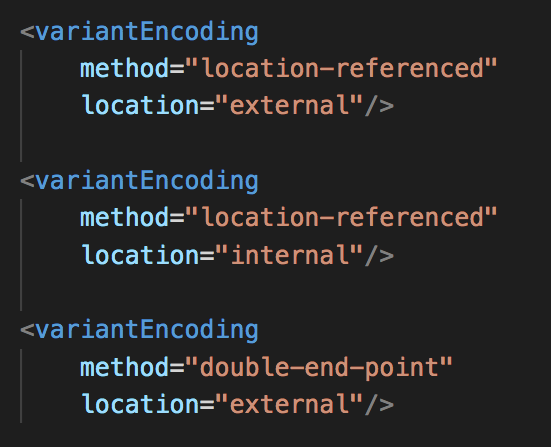
\includegraphics[width=.85\textwidth]{imgs/variantEncoding.png}
    \end{center}

\end{frame}



\begin{frame}
    \frametitle{TEI Modulo 12 - Codifica Edizioni Critiche}
    \framesubtitle{location-referenced method}
    \addtocounter{nframe}{1}
    
    % * Evidenziazione, page 17
    % The location-referenced method of encoding apparatus provides a convenient method for encoding printed apparatus

    % * Evidenziazione, page 17
    % the apparatus is linked to the base text by indicating explicitly only the block of text on which there is a variant

    % * Evidenziazione, page 17
    % usually by a canonical reference scheme, or by line number in the edition

    % * Evidenziazione, page 23
    % The location-referenced method can be used to point a position in a text using the @loc attribute and a canonical reference that is understood and documented in the context of the file where it is used

    \begin{block}{rappresentazione dell'apparato critico}
       %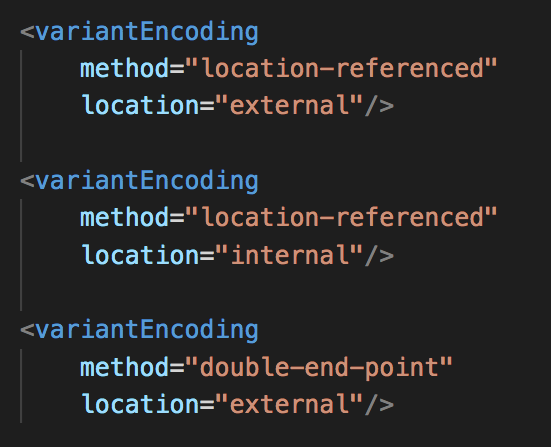
\includegraphics[width=.95\textwidth]{imgs/variantEncoding.png}
        Il metodo \textit{location-referenced} fornisce un approccio utile a codificare un apparato critico \textit{derivante da edizioni a stampa} o simile al modello di apparato a stampa
    \end{block}
    \begin{block}{rappresentazione dell'apparato critico}
         L'apparato è collegato al testo base indicando esplicitamente \textbf{solo il blocco di testo} (\textit{attraverso una forma canonica}) dove è presente la lettura divergente
     \end{block}

\end{frame}



\begin{frame}
    \frametitle{TEI Modulo 12 - Codifica Edizioni Critiche}
    \framesubtitle{location-referenced method}
    \addtocounter{nframe}{1}
    
    
        % * Evidenziazione, page 17
        % If the location-referenced method is used for an apparatus stored externally to the base text, the TEI header must have the declaration

        % * Evidenziazione, page 17
        % <variantEncoding method="location-referenced" location="external"/>

        % * Evidenziazione, page 17
        % In the body of the document, the base text (here El) will appear

        % * Evidenziazione, page 18
        % Elsewhere in the document, or in a separate file, the apparatus will appear

        % * Evidenziazione, page 18
        % On each app element, the @loc attribute should be specified to indicate where the variant occurs in the base text.

    \begin{center}
       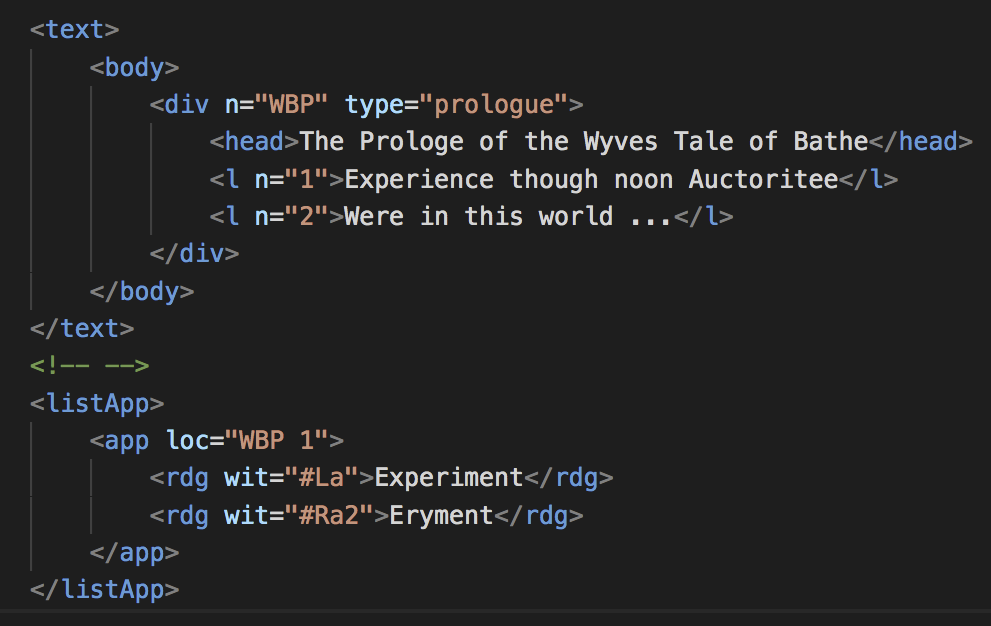
\includegraphics[width=.95\textwidth]{imgs/location-referenced.png}
    \end{center}

\end{frame}


\begin{frame}
    \frametitle{TEI Modulo 12 - Codifica Edizioni Critiche}
    \framesubtitle{location-referenced method}
    \addtocounter{nframe}{1}
    
    % * Evidenziazione, page 18
    % encoded using in-line storage

    % * Evidenziazione, page 18
    % apparatus is dispersed through the base text block to which it refers

    % * Evidenziazione, page 18
    % In this case, the location of the variant can be read from the line in which it occurs

    % * Evidenziazione, page 18
    % <variantEncoding method="location-referenced" location="internal"/>

    % * Nota ancorata, page 18
    % in-line location referenced method

    % Quando si registrano le varianti inline, il testo base va riportato fuori dall'apparato

    % * Evidenziazione, page 18
    % Since the location is not required to be exact, the apparatus for a line might also appear at the end of the line:

    % * Evidenziazione, page 18
    % <l n="1">Experience though noon Auctoritee <app> <rdg wit="#La"> Experiment</rdg> <rdg wit="#Ra2"> Eryment</rdg> </app> </l>

    % * Evidenziazione, page 18
    % it is not possible to find automatically the precise portion of text varied by the readings

    % * Evidenziazione, page 18
    % In order to show explicitly what portion of the base text is replaced by the variant readings, the lem element may be used:

    \begin{center}
       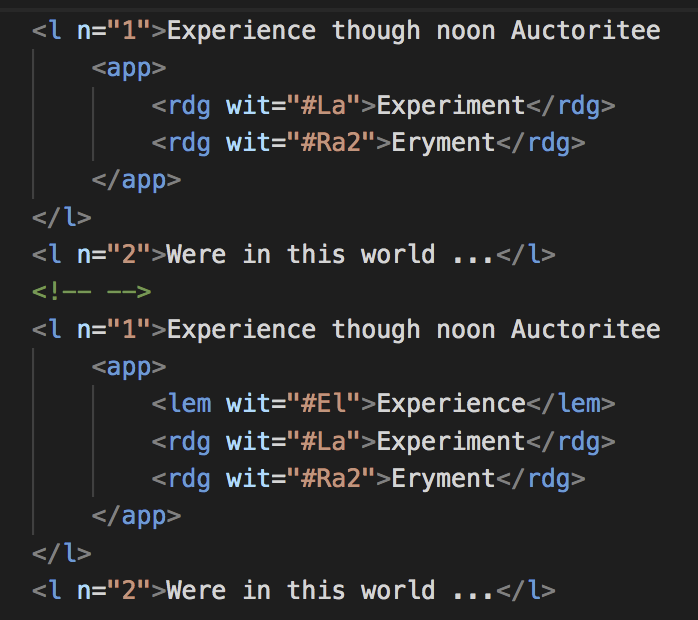
\includegraphics[width=.85\textwidth]{imgs/location-referenced-inline.png}
    \end{center}

\end{frame}

\begin{frame}
    \frametitle{TEI Modulo 12 - Codifica Edizioni Critiche}
    \framesubtitle{location-referenced method}
    \addtocounter{nframe}{1}
    
    % * Evidenziazione, page 19
    % no recommendations are made for conventions of abbreviating the lemma

    % * Evidenziazione, page 19
    % simple location-reference methods are unlikely to be as successful as the other two methods, which allow the unambiguous reconstruction of the lemma from the encoding.

    \begin{block}{Codifica dell'apparato critico}
       %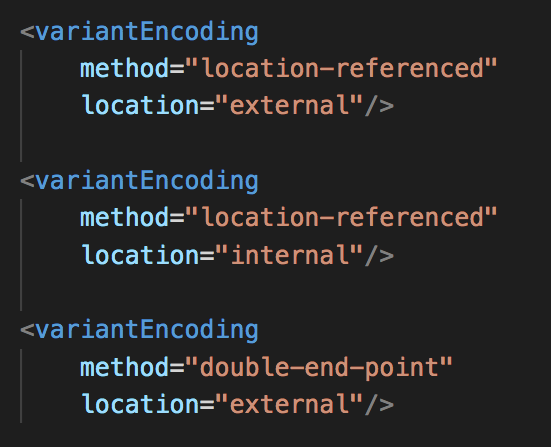
\includegraphics[width=.95\textwidth]{imgs/variantEncoding.png}
       Il metodo location-referenced non è consigliato per codificare entrate di apparato se sono previste elaborazioni automatiche poiché non prevede di esplicitare le letture divergenti collegandole all'esatta porzione del testo base.
    \end{block}

    \begin{center}
        \textit{I metodi Double End-Point Attachment e Parallel Segmentation sono più affidabili per eseguire successive elaborazioni sulle informazioni di apparato}
    \end{center}
    
\end{frame}



\begin{frame}
    \frametitle{TEI Modulo 12 - Codifica Edizioni Critiche}
    \framesubtitle{double end-point attachment method}
    \addtocounter{nframe}{1}
    
    % * Evidenziazione, page 19
    % In the double end-point attachment method, the beginning and end of the lemma in the base text are both explicitly indicated

    % * Evidenziazione, page 19
    % Double end-point attachment permits unambiguous matching of each variant reading against its lemma

    % * Evidenziazione, page 19
    % where the apparatus is intended to enable full reconstruction of the text

    \begin{block}{Estremi del lemma}
      Il metodo double end-point attachment \textbf{registra l'inizio e la fine del lemma all'interno del testo base}
    \end{block}
    
    \begin{block}{Associazione testo-varianti non ambigua}
        Grazie al collegamento puntuale ciascuna entrata di apparato seleziona in modo preciso la porzione di testo in oggetto, permettendo così la possibilità di ricostruire il testo di tutti i testimoni (\textit{apparato positivo}).
    \end{block}

\end{frame}




\begin{frame}
    \frametitle{TEI Modulo 12 - Codifica Edizioni Critiche}
    \framesubtitle{double end-point attachment method}
    \addtocounter{nframe}{1}
    
   % * Evidenziazione, page 19
    % the @from and @to attributes of the app element are used to indicate the beginning and ending points of the reading in the base text:

    % * Evidenziazione, page 19
    % identifiers which occur at the locations in question

    % * Evidenziazione, page 19
    % If no other markup is present there, the beginning and ending points should be marked using the anchor element

    \begin{block}{Attributi \texttt{@from} e \texttt{@to} dell'elemento \texttt{<app>}}
      Gli attributi \texttt{@from} e \texttt{@to} dell'elemento \texttt{<app>} sono usati per regitrare gli estremi (puntatori agli identificativi) di inizio e fine della lezione divergente rispetto alla lezione a testo
    \end{block}
    

\end{frame}


\begin{frame}
    \frametitle{TEI Modulo 12 - Codifica Edizioni Critiche}
    \framesubtitle{double end-point attachment method}
    \addtocounter{nframe}{1}
    
    % * Evidenziazione, page 19
    % The double end-point attachment method may be used with in-line or external apparatus

    % * Evidenziazione, page 19
    % the base text (here El) will appear with anchor elements inserted at every place where a variant begins or ends

    % * Evidenziazione, page 19
    % unless some element with an identifier already begins or ends at that point
   

    \begin{block}{apparato inline e external}
      Il metodo double end-point può essere implementato codificando l'apparato sia \textbf{in-line} (intercalato al testo base) sia \textbf{esternamente} (separato dal testo base anche in altro file)  
    \end{block}
    
    \begin{block}{Elemento \texttt{<anchor>}}
        Se non sono presenti elementi di annotazione per delimitare gli estremi della lezione, allora si utilizza l'elemento \texttt{<anchor>} intercalato al testo base.
     \end{block}

\end{frame}


\begin{frame}
    \frametitle{TEI Modulo 12 - Codifica Edizioni Critiche}
    \framesubtitle{double end-point attachment method}
    \addtocounter{nframe}{1}
    
    % * Evidenziazione, page 19
    % <variantEncoding method="double-end-point" location="external"/> <!-- ... --> <div n="WBP" type="prologue"> <head>The Prologe ... </head> <l n="1" xml:id="WBP.1">Experience<anchor xml:id="WBP-A2"/> though noon Auctoritee</l> <l>Were in this world ...</l> </div>

    % * Evidenziazione, page 19
    % separately encoded

    % * Evidenziazione, page 19
    % <app from="#WBP.1" to="#WBP-A2"> <rdg wit="#La">Experiment</rdg>

    % * Evidenziazione, page 20
    % <rdg wit="#Ra2">Eryment</rdg> </app>

    % * Evidenziazione, page 20
    % No anchor element is needed at the beginning of the line, since the @from attribute can use the identifier for the line as a whole

    % * Evidenziazione, page 20
    % the lemma is assumed to run from the beginning of the element indicated by the @from attribute, to the end of that indicated by the @to attribute
   
    \begin{center}
       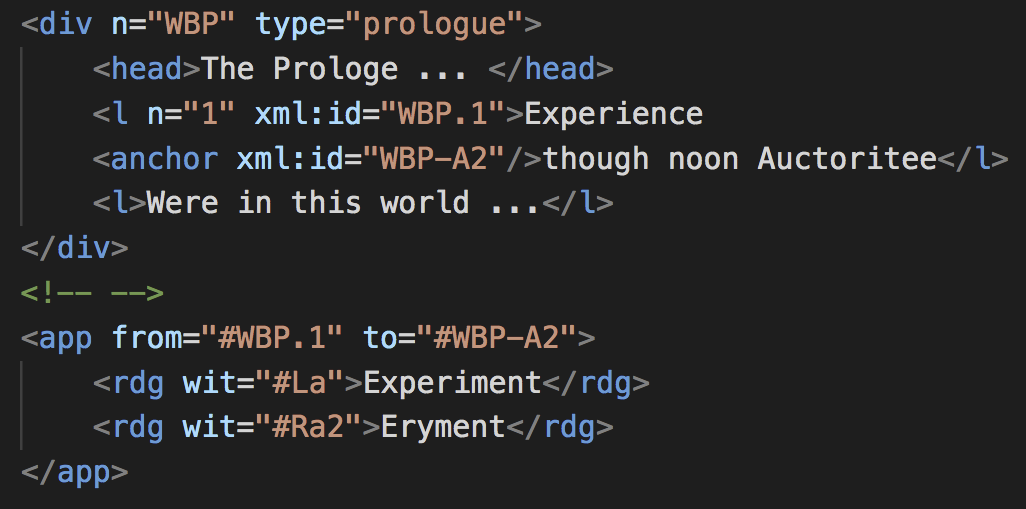
\includegraphics[width=.95\textwidth]{imgs/double-end-point.png}
    \end{center}

\end{frame}



\begin{frame}
    \frametitle{TEI Modulo 12 - Codifica Edizioni Critiche}
    \framesubtitle{double end-point attachment method}
    \addtocounter{nframe}{1}
    
    % * Evidenziazione, page 20
    % If no value is given for @to, the lemma runs from the beginning to the end of the element indicated by the @from attribute.

    % * Evidenziazione, page 20
    % When the apparatus is encoded in-line, it is dispersed through the base text

    % * Evidenziazione, page 20
    % Only the beginning of the lemma need be marked with an anchor, since the app is inserted at the end of the lemma, and itself therefore marks the end of the lemma.
   

    \begin{block}{Attributi \texttt{@from} e \texttt{@to}}
      Se non viene fornito alcun valore per l'attributo \texttt{@to}, allora il testo base selezionato è giudicato essere tutto il testo racchiuso nell'elemento indicato dall'attributo \texttt{@from}
    \end{block}
    
    \begin{block}{in-line double end-point}
       Se l'apparato è codificato inline, a quel punto solo l'inizio della lezione a testo deve essere contrassegnata: la fine è rappresentata dalla codifica dell'entrata di apparato.
    \end{block}

\end{frame}

\begin{frame}
    \frametitle{TEI Modulo 12 - Codifica Edizioni Critiche}
    \framesubtitle{double end-point attachment method}
    \addtocounter{nframe}{1}
    
    % * Evidenziazione, page 20
    % <variantEncoding method="double-end-point" location="internal"/> <!-- ... --> <l n="1" xml:id="wbp.1">Experience <app from="#wbp.1"> <rdg wit="#La">Experiment</rdg> <rdg wit="#Ra2">Eryment</rdg> </app> though noon Auctoritee</l> <l>Were in this world ...</l>
   
    \begin{center}
       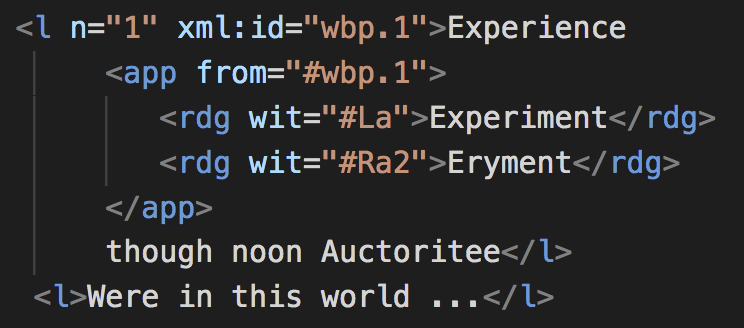
\includegraphics[width=.95\textwidth]{imgs/inline-double-end-point.png}
    \end{center}

\end{frame}

\begin{frame}
    \frametitle{TEI Modulo 12 - Codifica Edizioni Critiche}
    \framesubtitle{double end-point attachment method}
    \addtocounter{nframe}{1}
    % * Evidenziazione, page 20
    % The lemma need not be repeated within the app element in this method, as it may be extracted reliably from the base text

    % * Evidenziazione, page 20
    % if it is desired to make an explicit record of the attestation of the base text, the lem element may be embedded within app, carrying the witnesses to the base

    % * Evidenziazione, page 20
    % <app from="#WBP.1" to="#WBP-A2"> <lem wit="#El #Hg">Experience</lem>

    % * Evidenziazione, page 20
    % This method is designed to cope with ‘overlapping lemmata’

    % * Evidenziazione, page 21
    % This method can readily cope with such difficult situations

    % * Evidenziazione, page 21
    % typically found in large and complex traditions


    \begin{block}{Il lemma dell'apparato}
        Il metodo double end-point attachment non ha necessità di registrare la lezione a testo come lemma di apparato per ricostruire il testo
    \end{block}
    
    \begin{block}{gestione delle gerarchie sovrapposte}
       Il metodo double end-point attachment è progettato per gestire al meglio le \textbf{gerarchie sovrapposte} che possono presentarsi in grandi e complesse tradizioni testuali
    \end{block}

\end{frame}


\begin{frame}
    \frametitle{TEI Modulo 12 - Codifica Edizioni Critiche}
    \framesubtitle{double end-point attachment method}
    \addtocounter{nframe}{1}
    
    %% Gerarchie Sovrapposte %%
   
    \begin{center}
       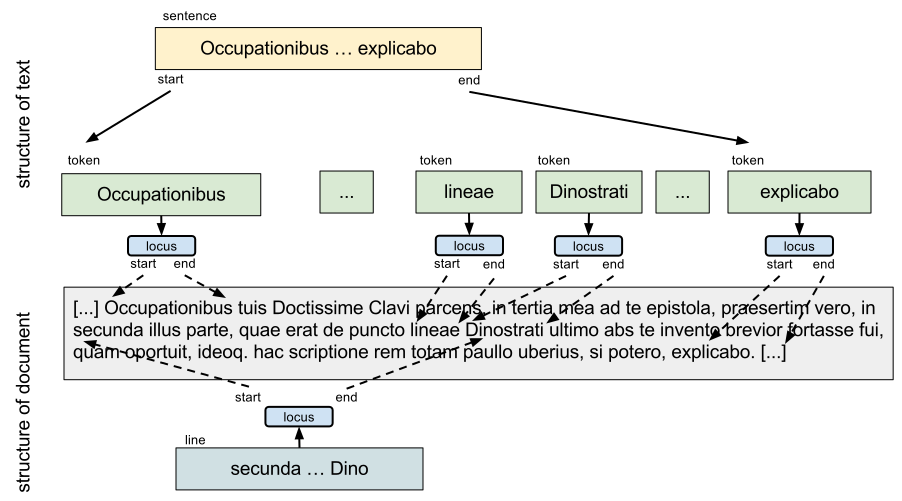
\includegraphics[width=.95\textwidth]{imgs/Clavius-DH.png}
    \end{center}

\end{frame}


\begin{frame}
    \frametitle{TEI Modulo 12 - Codifica Edizioni Critiche}
    \framesubtitle{double end-point attachment method}
    \addtocounter{nframe}{1}
   
    \begin{center}
       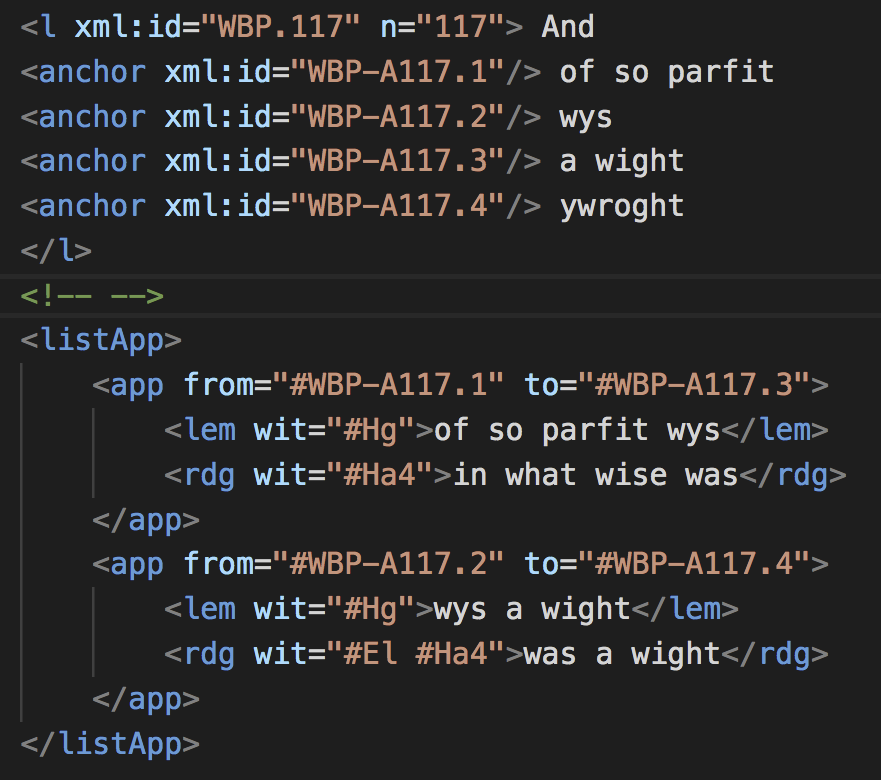
\includegraphics[width=.85\textwidth]{imgs/end-point-attachment-overlap.png}
    \end{center}

\end{frame}


\begin{frame}
    \frametitle{TEI Modulo 12 - Codifica Edizioni Critiche}
    \framesubtitle{double end-point attachment method}
    \addtocounter{nframe}{1}
    


% * Evidenziazione, page 19
% The beginning and end of the lemma may be indicated by using the ‘indirect pointing’ mechanisms

    \begin{block}{collegamento indiretto e stand-off}
      Se il testo base non può essere modificato e non ha le ancore per collegare l'entrata d'apparato con la lezione a testo, c'è la possibilità di sfruttare tecniche di collegamento indiretto in modalità stand-off
    \end{block}

    \textit{La stand-off annotation è una tecnica per tenere distinti su documenti o parti di documento differenti il testo e il suo insieme di annotazioni così che il legame fra i due sia stabilito tramite riferimenti univoci dalle annotazioni ai passi in oggetto, anche tramite espressioni indirette}

\end{frame}

\begin{frame}
    \frametitle{TEI Modulo 12 - Codifica Edizioni Critiche}
    \framesubtitle{double end-point attachment method}
    \addtocounter{nframe}{1}
    
   
    \begin{center}
       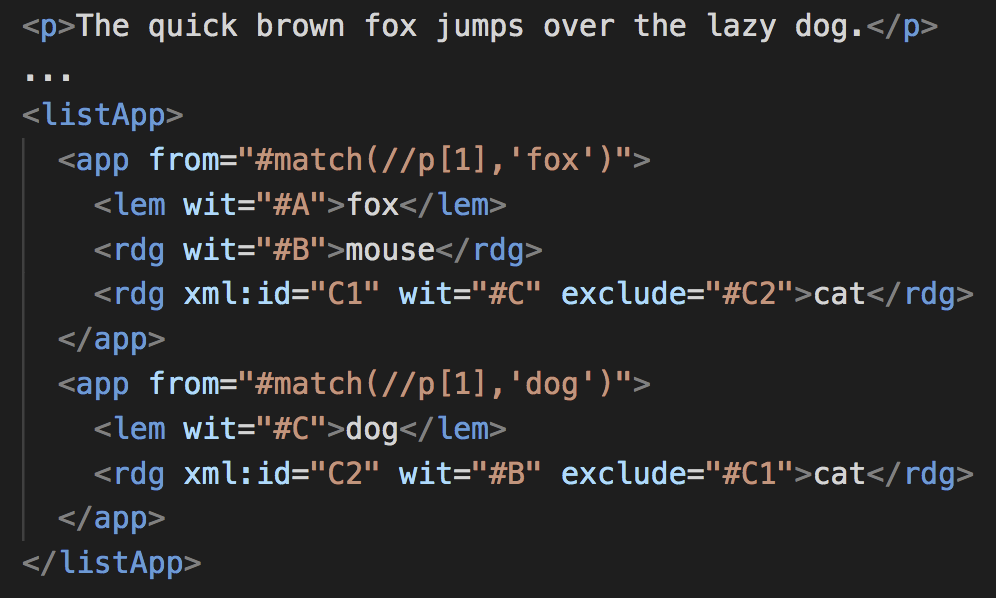
\includegraphics[width=.95\textwidth]{imgs/indirected-standoff-app.png}
    \end{center}

\end{frame}




\begin{frame}
    \frametitle{TEI Modulo 12 - Codifica Edizioni Critiche}
    \framesubtitle{parallel segmentation method}
    \addtocounter{nframe}{1}
    

    % The parallel segmentation method, to be discussed next, cannot handle overlaps among variants

    % * Evidenziazione, page 21
    % This method differs from the double end-point attachment method in that all variants at any point of the text are expressed as variants on one another.

    % * Evidenziazione, page 22
    % This method cannot be used with external apparatus

    % * Evidenziazione, page 22
    % it must be used in-line

    % * Evidenziazione, page 21
    % In this method, no two variations can overlap, although they may nest

    \begin{block}{Gerarchia sovrapposte e annidamenti}
      Il metodo parallel segmentation, a differenza degli altri metodi, gestisce tutti i luoghi del testo in cui si presentano lezioni divergenti come varianti l'una dell'altra registrate in-line.
    \end{block}

    \textbf{con il metodo parallel segmentation non è possibile gestire segmenti di testo divergente in sovrapposizione (overlap), ma i segmenti possono essere espressi tutt'al più con successive strutture gerarchiche perfettamente annidate}

\end{frame}

\begin{frame}
    \frametitle{TEI Modulo 12 - Codifica Edizioni Critiche}
    \framesubtitle{parallel segmentation method}
    \addtocounter{nframe}{1}
    
    % The parallel segmentation method does not use the concept of a base text and may only be used for in-line apparatus

    % * Evidenziazione, page 21
    % The texts compared are divided into matching segments all synchronized with one another

    % * Evidenziazione, page 21
    % It is also very easy with this method for an application to extract the full text of any one witness from the apparatus

    % * Evidenziazione, page 21
    % It will however be less convenient for very complex traditions

    % * Evidenziazione, page 21
    % In the parallel segmentation method, each segment of text on which there is variation is marked by an app element

    % * Evidenziazione, page 21
    % If there is a preferred (or base) reading it is tagged with lem; each reading is given in a rdg element:

    \begin{block}{segmenti e testo base}
      Il metodo parallel segmentation non ha il concetto di testo base, ma tutte le attestazioni divergenti sono registrate in apparato attraverso una oculata segmentazione dei passi con varianti mantenuti tra loro sincronizzati.
    \end{block}

    \textit{E' possibile estrarre il contenuto testuale di ciascun testimone selezionando uno specifico percorso, comprese le lezioni accettate dall'editore}

\end{frame}



\begin{frame}
    \frametitle{TEI Modulo 12 - Codifica Edizioni Critiche}
    \framesubtitle{parallel segmentation method}
    \addtocounter{nframe}{1}
    
    % * Evidenziazione, page 22
    % the witnesses to the reading most widely attested need not be stated

    % * Evidenziazione, page 22
    % read a listWit declaring all the witnesses to the text and then calculate which witnesses have not been named

    % * Evidenziazione, page 22
    % To avoid confusion, however, witnesses may be omitted only for a single reading.

    % * Evidenziazione, page 22
    % <l n="1"> <app> <lem>Experience</lem> <rdg wit="#La">Experiment</rdg> <rdg wit="#Ra2">Eryment</rdg> </app> though noon Auctoritee </l>

   
    \begin{center}
       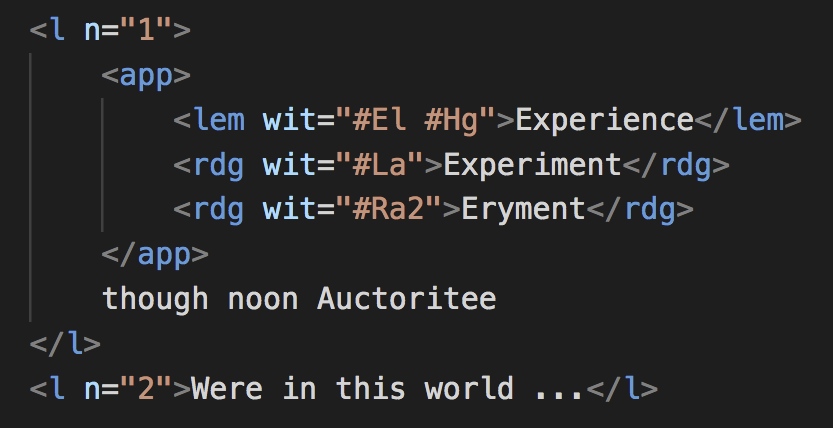
\includegraphics[width=.95\textwidth]{imgs/parallel-segmentation.png}
    \end{center}

\end{frame}



\begin{frame}
    \frametitle{TEI Modulo 12 - Codifica Edizioni Critiche}
    \framesubtitle{parallel segmentation method}
    \addtocounter{nframe}{1}

    % * Evidenziazione, page 22
    % apparatus entries may nest in this method

    % * Evidenziazione, page 22
    % the variation on the individual words of the line would nest within that for the line as a whole:


    % * Evidenziazione, page 23
    % Parallel segmentation cannot, however, deal very gracefully with variants which overlap without nesting
   
    \begin{center}
       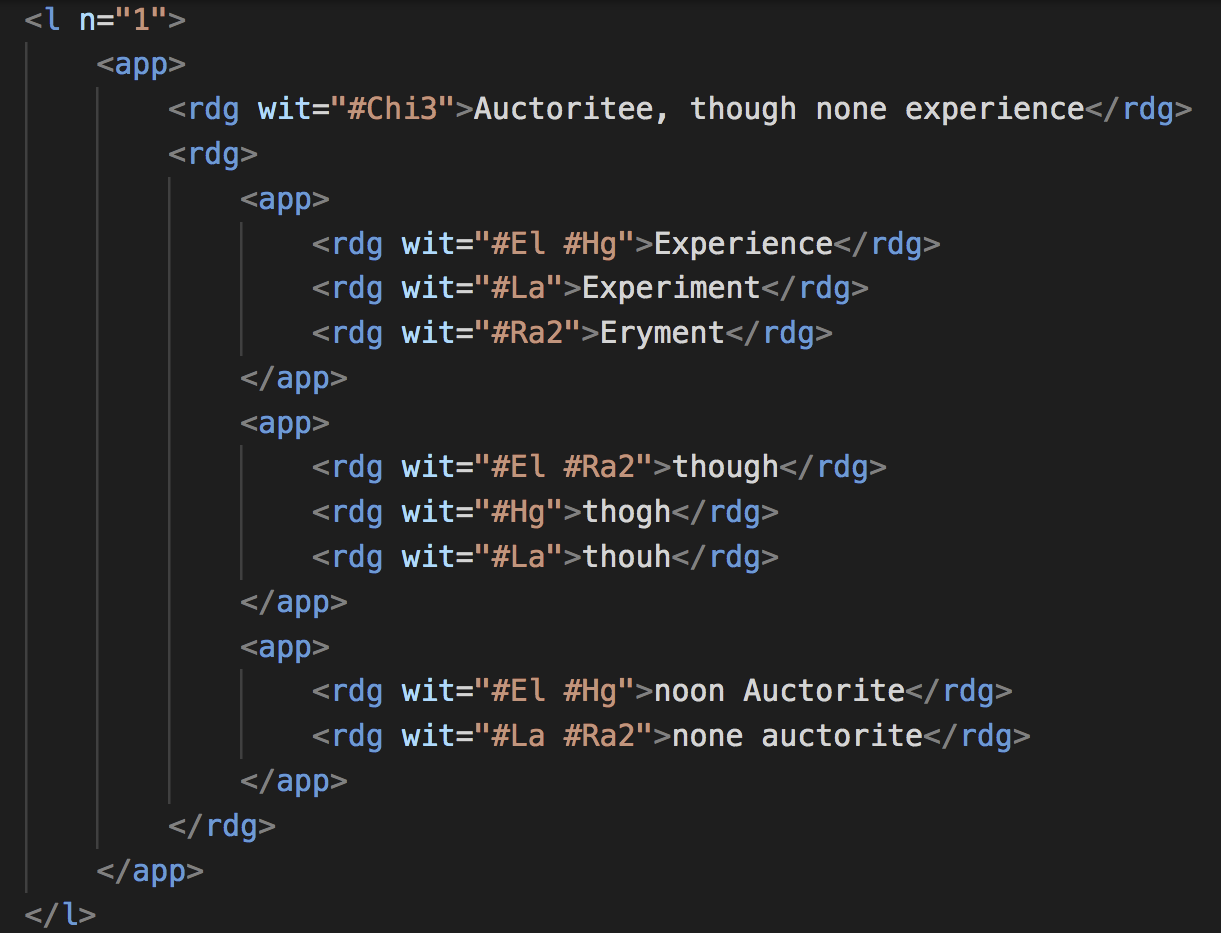
\includegraphics[width=.90\textwidth]{imgs/parallel-segmentation-nested.png}
    \end{center}

\end{frame}


\begin{frame}
    \frametitle{TEI Modulo 12 - Codifica Edizioni Critiche}
    \framesubtitle{}
    \addtocounter{nframe}{1}
    
    % * Evidenziazione, page 23
    % When an apparatus is provided it does not need to be given at the location in the transcription where the variation, emendation, attribution, or other apparatus observation occurs. Instead it may be stored in a separate place in the same file, or indeed in another file, and point to the location at which it is meant to be used

    % * Evidenziazione, page 23
    % The @from attribute is a data.pointer datatype and thus contains a URI as a value

    %directly to an @xml:id, an @xml:id in another local file, or indeed a file identified by any URL or URN

    \begin{block}{Collegamento dell'entrata di apparato con URI}
       %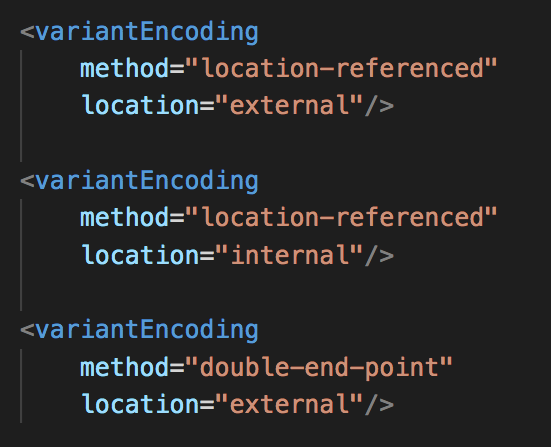
\includegraphics[width=.95\textwidth]{imgs/variantEncoding.png}
       L'attributo @from può assumere come valori tipi di dato riconducibili agli URI (Uniform Resurce Identifier)
    \end{block}
    \textbf{Collegamenti ad elementi tramite xml:id in uno stesso file, in file diversi in locale, in file diversi remoti con URL oppure URN}

\end{frame}



\begin{frame}
    \frametitle{TEI Modulo 12 - Codifica Edizioni Critiche}
    \framesubtitle{}
    \addtocounter{nframe}{1}
    
    % * Evidenziazione, page 23
    % Where possible it is recommended that other methods use the @from attribute to point to an @xml:id attribute on an anchor or other element at the location where the apparatus observation takes place

    % * Evidenziazione, page 23
    % The contents of an element pointed to are understood to be equivalent to a lem if none exists in the app, and if a lem does exist this should replace any content.

    \begin{center}
       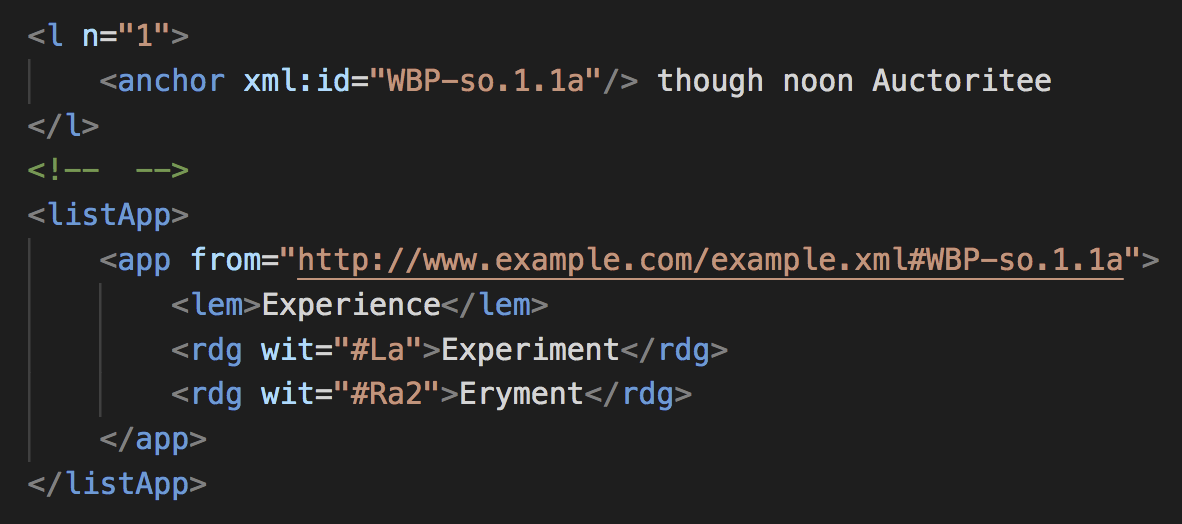
\includegraphics[width=.95\textwidth]{imgs/app-uri-png.png}
    \end{center}
   
\end{frame}



\begin{frame}
    \frametitle{TEI Modulo 12 - Codifica Edizioni Critiche}
    \framesubtitle{}
    \addtocounter{nframe}{1}
    
    % * Evidenziazione, page 24
    % In addition, URLs can contain XPointer schemes including xpath(), range(), and string-range() which can be used in providing the location of an app that is stored separately from the text to which it applies

    % * Evidenziazione, page 24
    % Both @from and @to can be used, as in the double end-point attachment method, to identify the starting and ending location for an apparatus using XPointer schemes described

    \begin{block}{Collegamento con schemi XPointer}
       Oltre ad impiegare identificativi URI è possibile selezionare la porzione di testo base sfruttando schemi Xpointer
    \end{block}
    \textbf{Funzioni XPointer quali xpath(), range(), and string-range()}

\end{frame}



\begin{frame}
    \frametitle{TEI Modulo 12 - Codifica Edizioni Critiche}
    \framesubtitle{}
    \addtocounter{nframe}{1}

    % * Evidenziazione, page 24
    % If only the @from attribute is provided then it should be understood that this supplies the location of the textual variance that the apparatus documents

    % * Evidenziazione, page 24
    % If the @from attribute contains an XPointer scheme that identifies a range of text

    % * Evidenziazione, page 24
    % record the starting and ending of the range

    % * Evidenziazione, page 24
    % In such a case a @to attribute is unnecessary.
    
    \begin{center}
       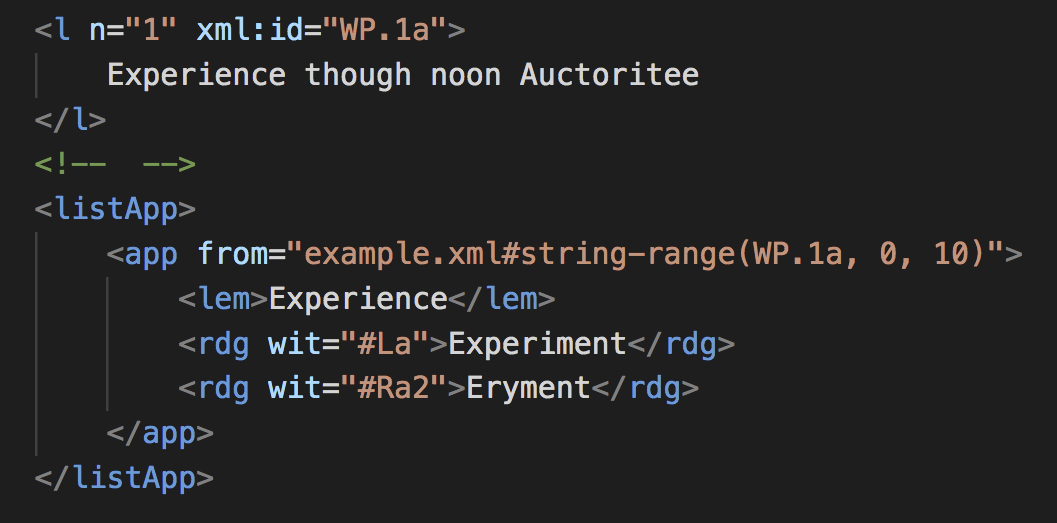
\includegraphics[width=.95\textwidth]{imgs/app-xpointer.png}
    \end{center}
   
\end{frame}



\begin{frame}
    \frametitle{TEI Modulo 12 - Codifica Edizioni Critiche}
    \framesubtitle{record different transcriptions}
    \addtocounter{nframe}{1}
    
    % * Evidenziazione, page 24
    % It is often desirable to record different transcriptions of one stretch of text.

    % * Evidenziazione, page 24
    % An application may then construct different ‘views’ of the transcription by extraction of the appropriate variant readings from the apparatus elements embedded in the transcription.

    % * Evidenziazione, page 24
    % For example, alternative expansions can be recorded in several different expan elements, all grouped within an app element

    % * Evidenziazione, page 24
    % which has been read in different ways by different scholars

    % * Evidenziazione, page 25
    % In most cases, elements used to indicate features of a primary textual source may be represented within an app structure simply by nesting them within its readings

    % * Evidenziazione, page 25
    % the markup may use the join element or the @next and @prev attributes defined by chapter


    \begin{block}{Varianti in trascrizione}
       %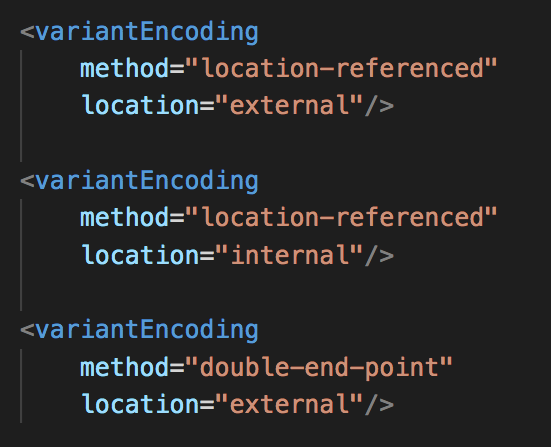
\includegraphics[width=.95\textwidth]{imgs/variantEncoding.png}
       Spesso si vuole registrare diverse possibili trascrizioni di uno stesso passo testuale. In questo modo è possibile ricostruire diverse versioni di una stessa fonte primaria con diverse interpretazioni nella trascrizione.
    \end{block}
    \textit{Per esempio differenti versioni per lo scioglimento di abbreviazioni lette da diversi studiosi}

\end{frame}


\begin{frame}
    \frametitle{TEI Modulo 12 - Codifica Edizioni Critiche}
    \framesubtitle{record different transcriptions}
    \addtocounter{nframe}{1}
    
    % * Evidenziazione, page 24
    % This information may be held within an app structure

    % * Evidenziazione, page 24
    % <app> <rdg source="#ES">perfectio<am> <g ref="#ii"/> </am> </rdg> <rdg source="#FJF">perfectio<ex>u</ex>n</rdg> <rdg source="#PGR">perfectiou<ex>n</ex>

    % * Evidenziazione, page 25
    % Editorial notes may also be attached to app structures within transcriptions

    \begin{center}
       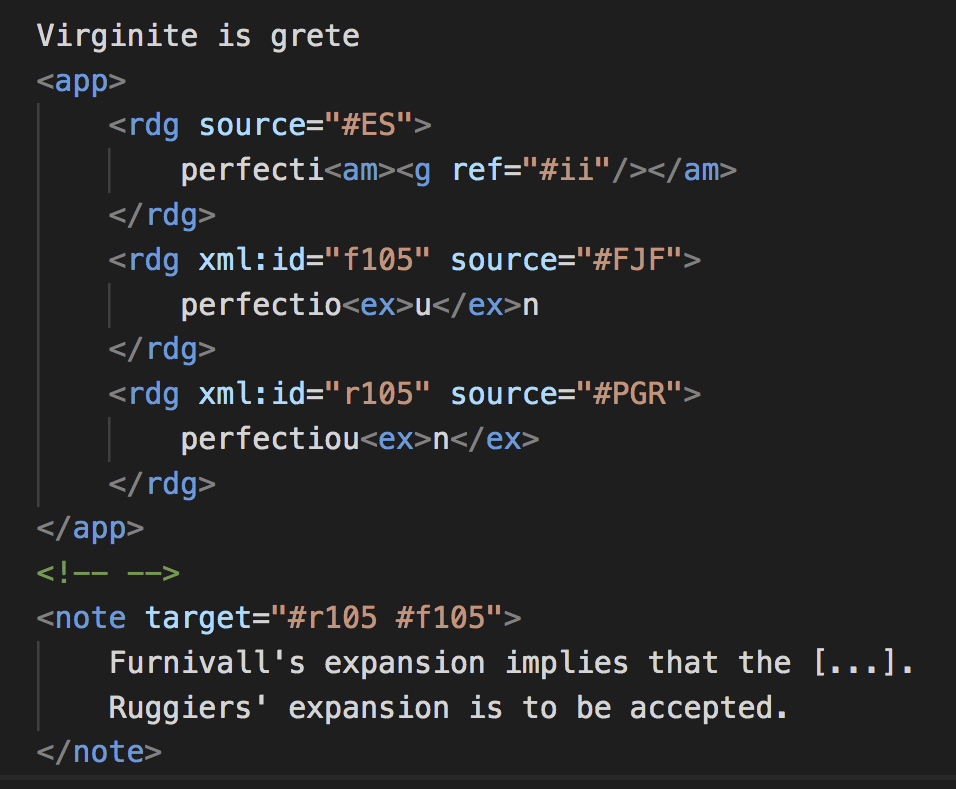
\includegraphics[width=.85\textwidth]{imgs/app-trascrizion-note.png}
    \end{center}

\end{frame}



\begin{frame}
    \frametitle{TEI Modulo 12 - Codifica Edizioni Critiche}
    \framesubtitle{Strategies for Encoding Variation}
    \addtocounter{nframe}{1}
    
    % * Evidenziazione, page 26
    % Phenomena such as omissions and transpositions in witnesses will require some encoding strategies that differ from those in the examples above

    % * Evidenziazione, page 25
    % some care must be taken in their encoding to ensure that TEI's Abstract Model is not being broken.

    % * Evidenziazione, page 26
    % Similarly, it is an error if the contents of an apparatus entry place a p inside another p or an l inside an l.

    \begin{block}{fenomeni critici}
       %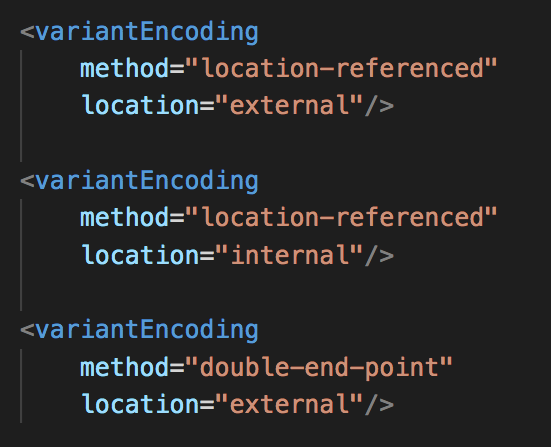
\includegraphics[width=.95\textwidth]{imgs/variantEncoding.png}
       Fenomeni quali omissioni, trasposizioni, contaminazioni, omeoarchie necessitano di particolare cura per la loro corretta codifica
    \end{block}
    \textbf{attenzione a non "\textit{rompere}" il modello astratto della struttura TEI (\textit{es. sostituire un paragrafo con un verso in una strofa di poesia})}

\end{frame}

\begin{frame}
    \frametitle{TEI Modulo 12 - Codifica Edizioni Critiche}
    \framesubtitle{Strategies for Encoding Variation}
    \addtocounter{nframe}{1}
    
    % * Evidenziazione, page 25
    % Variation most frequently occurs at the phrase level, but is also common at higher structural levels, such as the verse line, paragraph, or chapter

    % * Evidenziazione, page 26
    % An editor wishing to signal an omission in one witness should encode the omission using an empty rdg

    % * Evidenziazione, page 26
    % <app xml:id="d1e372"> <lem xml:id="d1e373" source="#Heyworth"> <l n="18">Hypsipyle uacuo constitit in thalamo:</l> </lem> <rdg xml:id="d1e376" wit="#J" cause="homeoarchon"/> </app> 
    %omeoarchia % contaminatio % interpolazione

    % * Evidenziazione, page 26
    % Notice that in this example, the variation occurs at the unit of the verse line

    % * Evidenziazione, page 26
    % by mistake

    % * Evidenziazione, page 26
    % If a witness contains an interpolation that the editor does not wish to show in the base text, an empty lem should be used, in the same fashion.

    \begin{center}
       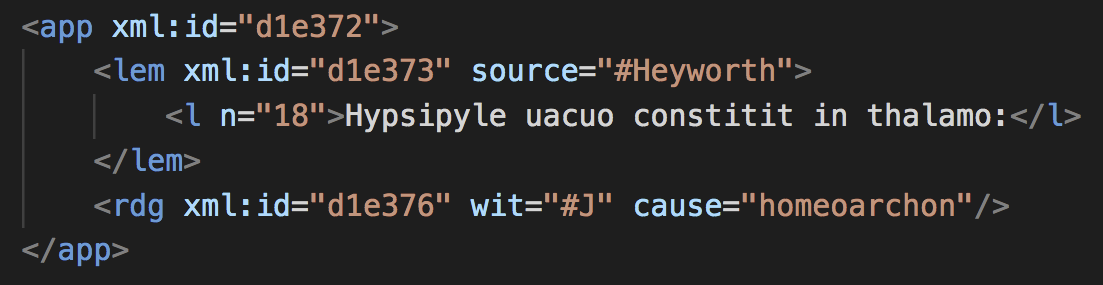
\includegraphics[width=.95\textwidth]{imgs/app-omeoarchia.png}
    \end{center}

\end{frame}




\begin{frame}
    \frametitle{TEI Modulo 12 - Codifica Edizioni Critiche}
    \framesubtitle{Strategies for Encoding Variation}
    \addtocounter{nframe}{1}
    
    % * Evidenziazione, page 26
    % Transpositions are harder to encode

    % * Evidenziazione, page 26
    % A single app will therefore not be sufficient

    % * Evidenziazione, page 26
    % and the variants must be linked.
    
    % * Evidenziazione, page 26
    % Note that both apps are linked via the @exclude attribut
    
    % * Evidenziazione, page 26
    % because they are mutually exclusive

    \begin{block}{trasposizioni}
       %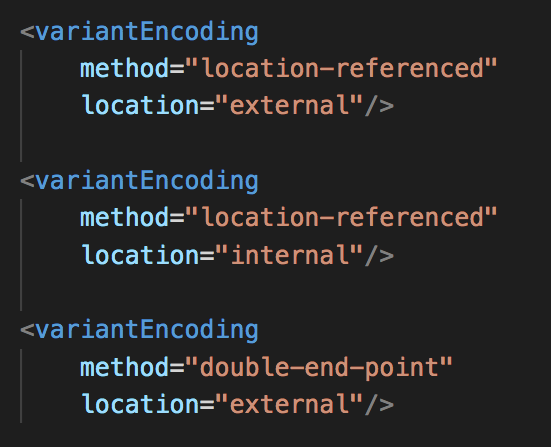
\includegraphics[width=.95\textwidth]{imgs/variantEncoding.png}
       Rappresentare in TEI le trasposizioni non è affatto banale. Generalmente bisogna ricorrere a strategie verbose e trucchetti.
    \end{block}
    \textbf{Usare più entrate d'apparato, copie di elementi e attributi di mutua esclusione}

\end{frame}


\begin{frame}
    \frametitle{TEI Modulo 12 - Codifica Edizioni Critiche}
    \framesubtitle{Strategies for Encoding Variation}
    \addtocounter{nframe}{1}
    
    % * Evidenziazione, page 26
    % To avoid repetition, the second pair of lines can make use of the @copyOf attribute.

    % * Evidenziazione, page 26
    % Apparatus entries may nest when there is variation at both higher and lower structural levels


    \begin{center}
       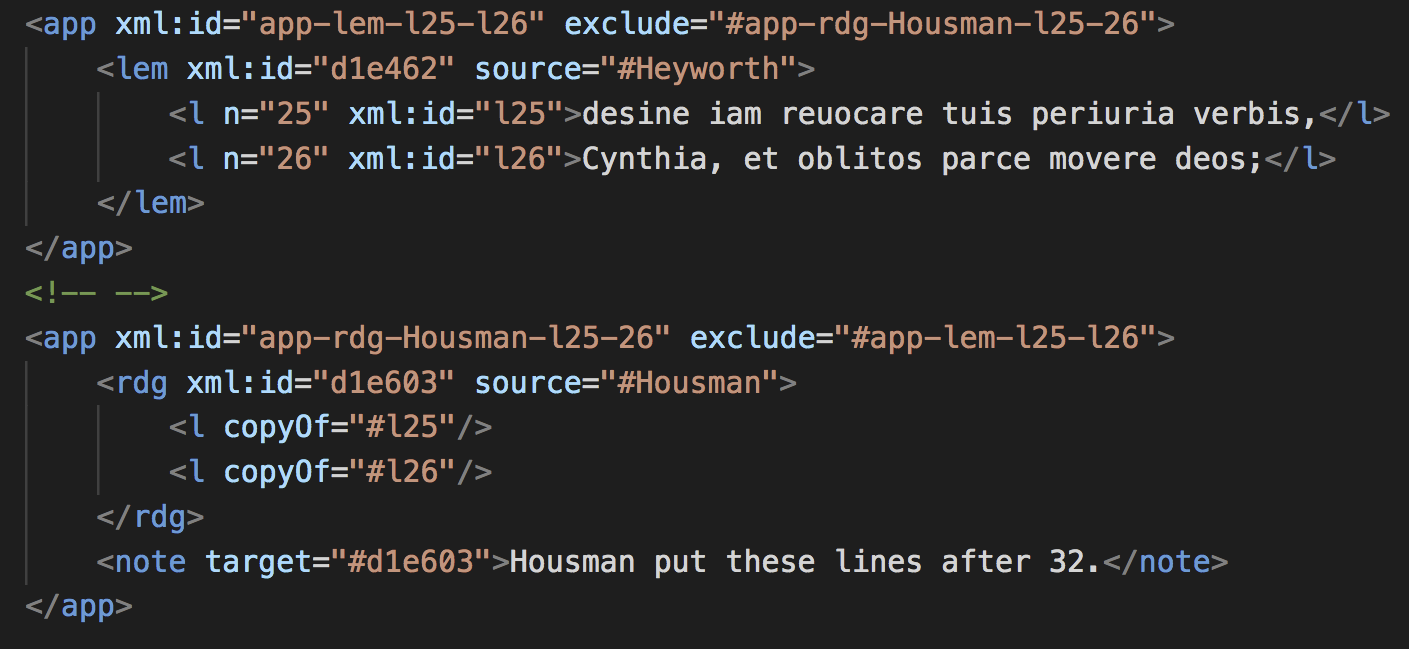
\includegraphics[width=.95\textwidth]{imgs/app-transposition.png}
    \end{center}

\end{frame}


% * Evidenziazione, page 27
% <app xml:id="d1e275"> <lem xml:id="d1e277" source="#Heyworth"> <l n="8"> <app xml:id="d1e280"> <lem xml:id="d1e281" wit="#N #Λ">ut</lem> <rdg xml:id="d1e283" wit="#A">et</rdg> <rdg xml:id="d1e285" source="#Nodell">ac</rdg> <note target="#d1e287">perhaps</note> <rdg xml:id="d1e287" source="#Heyworth" cert="low">quam</rdg> </app> formosa nouo quae parat ire uiro.</l> <l n="9"> <app xml:id="d1e294"> <lem xml:id="d1e295">at</lem> <rdg xml:id="d1e297" wit="#A">et</rdg> </app> non sic, Ithaci digressu <app xml:id="d1e300"> <lem xml:id="d1e301">mota</lem> <rdg xml:id="d1e303" source="#Graevius">immota</rdg> </app>, Calypso</l> <l n="10">desertis olim fleuerat aequoribus:</l> <l n="11">multos illa dies incomptis maesta capillis</l> </lem> <rdg xml:id="d1e314" wit="#C" cause="homoeoteleuton"/> <note target="#d1e314">omits lines 8-11 because of homoeoteleuton.</note> </app>

% * Evidenziazione, page 27
% Here, MS C omits lines 8-11, but there are variations the editor wishes to record in the other witnesses which do have these lines

% * Evidenziazione, page 27
% Therefore, an outer app gives the lines in the lem and the omission in a rdg

% * Evidenziazione, page 27
% Further variation is encoded for lines 8 and 9 using nested apps.





% This panel addresses the TEI critical apparatus as a data model, investigating how it has expanded the capacity of scholarly editions to articulate and analyze phenomena of textual variation and multiplicity. We will discuss how the TEI critical apparatus, as a structure that mediates distinct versions of a work, is expanding horizons for multidimensional and pluralistic document modeling. Our panel surveys recent experiments with the critical apparatus that have led to new kinds of scholarly research and in some cases to revisions to the TEI Guidelines. What kinds of research questions and applications can we support with the TEI critical apparatus, and what practical challenges do we face in working with it in inline and stand-off ways? We begin by investigating how the TEI critical apparatus has transformed the expressive capacity of scholarly editions to prioritize textual multiplicity. We continue by sharing data models that apply TEI critical apparatus as a stand-off “spine” for connecting independently encoded witnesses. We conclude by inviting the audience to discuss with us the scalability of these methods for texts with large numbers of witnesses, and the technological challenges and opportunities of stand-off methods in light of recent changes to the TEI Guidelines. 

% What *really* is a critical apparatus (James Cummings)